%%%%%%%%%%%%%%%%%%%%%%%%%%%%%%%%%%%%%%%%%%%%%%%%%%%%%%%
%% Bachelor's & Master's Thesis Template             %%
%% Copyleft by Artur M. Brodzki & Piotr Woźniak      %%
%% Faculty of Electronics and Information Technology %%
%% Warsaw University of Technology, 2019-2020        %%
%%%%%%%%%%%%%%%%%%%%%%%%%%%%%%%%%%%%%%%%%%%%%%%%%%%%%%%

\documentclass[
    left=2.5cm,         % Sadly, generic margin parameter
    right=2.5cm,        % doesnt't work, as it is
    top=2.5cm,          % superseded by more specific
    bottom=3cm,         % left...bottom parameters.
    bindingoffset=6mm,  % Optional binding offset.
    nohyphenation=false % You may turn off hyphenation, if don't like.
]{eiti/eiti-thesis}

\usepackage{silence}
\WarningFilter{caption}{Unknown document class}

\ifluatex
    \pdfvariable minorversion 7
\fi

\usepackage{etoolbox}

\usepackage{fontspec}
\setmainfont{texgyretermes}[
  Extension      = .otf ,
  UprightFont    = *-regular ,
  ItalicFont     = *-italic ,
  BoldFont       = *-bold ,
  BoldItalicFont = *-bolditalic ,
]

\langpol % Dla języka angielskiego mamy \langeng
\graphicspath{{img/}}             % Katalog z obrazkami.
\addbibresource{bibliografia.bib} % Plik .bib z bibliografią

\usepackage{xurl} % Pozwala na łamanie URL w dowolnym miejscu

\usepackage{float}
\usepackage{listings}
\usepackage{xcolor}
\usepackage{tcolorbox}
\tcbuselibrary{breakable, skins}

\newtcolorbox{techcard}[1]{
    enhanced,
    title={\textbf{Karta narzędzia: }#1},
    colback=gray!5,
    colframe=black!50,
    coltitle=black,
    fonttitle=\bfseries,
    breakable,
    before skip=\medskipamount,
    after skip=\medskipamount,
}

\lstset{
    basicstyle=\ttfamily\footnotesize,
    breaklines=true,
    breakatwhitespace=false,
    frame=single,
    numbers=left,
    numberstyle=\tiny\color{gray},
    stepnumber=1,
    tabsize=2,
    showstringspaces=false,
    captionpos=b,
}

\lstdefinelanguage{yaml}{
  keywords={true,false,null,yes,no},
  keywordstyle=\color{blue}\bfseries,
  sensitive=false,
  comment=[l]{\#},
  commentstyle=\color{gray}\ttfamily,
  stringstyle=\color{teal}\ttfamily,
  morestring=[b]',
  morestring=[b]",
}

\lstdefinelanguage{docker}{
  keywords={FROM,RUN,CMD,LABEL,EXPOSE,ENV,ADD,COPY,ENTRYPOINT,VOLUME,USER,WORKDIR,ARG,ONBUILD,STOPSIGNAL,HEALTHCHECK,SHELL,AS},
  keywordstyle=\color{blue}\bfseries,
  sensitive=true,
  comment=[l]{\#},
  commentstyle=\color{gray}\ttfamily,
  stringstyle=\color{teal}\ttfamily,
  morestring=[b]',
  morestring=[b]",
}

\lstdefinelanguage{groovy}{
  keywords={def,class,interface,extends,implements,return,if,else,for,while,
            try,catch,finally,throws,new,void,true,false,null,import,package,
            static,public,private,protected,final,abstract,
            plugins,dependencies,id,implementation,testImplementation,
            runtimeOnly,compileOnly,annotationProcessor,
            quarkusBuild,nativeArgs,containerBuild,builderImage,
            repositories,mavenCentral,mavenLocal,group,version,apply},
  keywordstyle=\color{blue}\bfseries,
  sensitive=true,
  comment=[l]{//},
  comment=[s]{/*}{*/},
  commentstyle=\color{gray}\ttfamily,
  stringstyle=\color{teal}\ttfamily,
  morestring=[b]',
  morestring=[b]",
}

% Poprawa łamania linii w bibliografii
\appto{\bibsetup}{
    \setcounter{biburllcpenalty}{7000}
    \setcounter{biburlucpenalty}{8000}
    \setcounter{biburlnumpenalty}{9000}
    \emergencystretch=3em
    \sloppy
}

\raggedbottom

\begin{document}

%--------------------------------------
% Strona tytułowa
%--------------------------------------
\EngineerThesis % Dla pracy inżynierskiej mamy \EngineerThesis
\instytut{Telekomunikacji}
\kierunek{Elektronika i Telekomunikacja}
\specjalnosc{Teleinformatyka}
\title{
    DevOps – przegląd i implementacja dobrych praktyk nowoczesnego wytwarzania oprogramowania
}
\engtitle{ % Tytuł po angielsku do angielskiego streszczenia
    DevOps – review and implementation of modern software development good practices
}
\author{Mateusz Waś}
\album{217860}
\promotor{dr inż. Maciej Sosnowski}
\date{\the\year}
\maketitle

%--------------------------------------
% Streszczenie po polsku
%--------------------------------------
\cleardoublepage % Zaczynamy od nieparzystej strony
\streszczenie{
Ta praca skupia się na prezentacji dobrych praktyk w projektowaniu i wytwarzaniu oprogramowania w oparciu o metodykę DevOps i podejście Cloud Native. Przykładem jest projekt serwisu oparty na architekturze mikrousługowej, który prezentuje krok po kroku idee "pętli ciągłego rozwoju" zaczerpniętej z DevOps oraz konkretne narzędzia, które można wykorzystać na każdym etapie. Jest to praktyczny przykład architektury nowoczesnego systemu aplikacyjnego, który opiera się na mikroserwisach, konteneryzacji i orkiestracji na platformie Kubernetes. Na podstawie realnych przykładów, ta praca dostarcza czytelnikowi konkretnych wskazówek i rozwiązań na drodze do pomyślnego wdrożenia narzędzi DevOps w swoim projekcie.
}
\slowakluczowe DevOps, Cloud Native, Kubernetes, automatyzacja, dobre praktyki,  projektowanie systemów, pętla ciągłego rozwoju

%--------------------------------------
% Streszczenie po angielsku
%--------------------------------------
\newpage
\abstract{
The thesis illustrates best practices in software design and implementation, thorough the lens of DevOps methodology and Cloud Native principles. Using a microservices project as a practical example it demonstrates each step of the DevOps continuous improvement loop. By showcasing the relevant tools for each project stage, it offers a hands-on look at modern system software design centered around microservices, containerization and Kubernetes. By providing real-world examples, this research equips readers with valuable insights and actionable guidance for adopting and implementing DevOps tools effectively in their own projects.
}
\keywords DevOps, Cloud Native, Kubernetes, automation, best practices, system design, continuous improvement loop

%--------------------------------------
% Oświadczenie o autorstwie
%--------------------------------------
\cleardoublepage  % Zaczynamy od nieparzystej strony
\pagestyle{plain}
\makeauthorship

%--------------------------------------
% Spis treści
%--------------------------------------
\cleardoublepage % Zaczynamy od nieparzystej strony
\tableofcontents

%--------------------------------------
% Rozdziały
%--------------------------------------
\cleardoublepage % Zaczynamy od nieparzystej strony
\pagestyle{headings}

\newpage
\section{Wstęp}
\subsection{Wprowadzenie}
Współcześnie coraz częściej używa się terminu \textit{Cyfrowa Gospodarka} i \textit{Gospodarka 4.0} by pokazać wpływ technologii informacyjnych na naszą codzienność. Oprogramowanie wspomaga nas w wielu dziedzinach życia, a pandemia COVID-19 bardzo przyśpieszyła proces cyfrowej transformacji \cite{Sledziewska2021DigitalTransformation} \cite{Grande2024DevOpsGlobalSoftware}.

\noindent Cyfrowe usługi dostępne są w najróżniejszych gałęziach gospodarki, w tym:
\begin{itemize}
    \item \textbf{Przemysł i produkcja:} Automatyzacja, robotyka i Internet Rzeczy (IoT) zmieniają sposób, w jaki produkty są wytwarzane, kontrolowane i monitorowane.
    \item \textbf{Handel elektroniczny:} Sklepy internetowe, platformy zakupowe i płatności elektroniczne pozwalają na handel bezpośrednio przez internet, przekształcając tradycyjne modele handlu.
    \item \textbf{Usługi finansowe:} Technologie FinTech, takie jak mobilne aplikacje bankowe, kryptowaluty i rozwiązania oparte na blockchainie, zmieniają sposób, w jaki ludzie zarządzają finansami i inwestują.
    \item \textbf{Edukacja:} E-learning, platformy online i narzędzia edukacyjne umożliwiają zdalne kształcenie i dostęp do wiedzy na skalę globalną.
    \item \textbf{Opieka zdrowotna:} Telemedycyna, zdalne monitorowanie pacjentów i analiza danych przyczyniają się do poprawy dostępu do opieki zdrowotnej i skracają czas diagnostyki.
    \item \textbf{Komunikacja społeczna:} Media społecznościowe i platformy komunikacyjne umożliwiają ludziom interakcję, udostępnianie treści oraz tworzenie społeczności online.
    \item \textbf{Praca zdalna:} Rozwój narzędzi do pracy zdalnej i współpracy online zmienia tradycyjne modele pracy, umożliwiając elastyczność i globalną współpracę.
    \item \textbf{Transport i logistyka:} Aplikacje do zamawiania taksówek, dostaw żywności i usług kurierskich rewolucjonizują branżę transportową i logistyczną.
    \item \textbf{Rozrywka i kultura:} Strumieniowanie muzyki, filmów, gier i treści multimedialnych stało się integralną częścią cyfrowej kultury.
    \item \textbf{Badania naukowe:} Analiza dużych zbiorów danych, obliczenia rozproszone i symulacje komputerowe przyczyniają się do postępu naukowego w wielu dziedzinach.
\end{itemize}
Coraz większe wymagania użytkowników co do usług cyfrowych --- ich dostępności, stabilności, rozwoju, jakości i przydatności --- sprawiają, że firmy technologiczne muszą szukać sposobów na optymalizację procesu wytwarzania oprogramowania.
Jako główne cele stawia się, m.in.: elastyczność; skalowalność; szybkość wdrożeń; odporność na awarie; automatyzację; wsparcie dla innowacji; dostępność i globalny dostęp; redukcję kosztów; bezpieczeństwo i ochronę danych; zrównoważony rozwój; łatwą współpracę i udostępnianie treści.

W wyniku coraz większego zapotrzebowania zmieniają się też metodyki wytwarzania oprogramowania. Wśród nich można wyróżnić kilka skupionych na wykorzystaniu skalowalności systemów chmur obliczeniowych:

\subsubsection{The Twelve-Factor App}
Metodologia Twelve-Factor App to zbiór dwunastu zasad opracowanych przez inżynierów z firmy Heroku, które mają na celu ułatwienie tworzenia nowoczesnych, skalowalnych i łatwych w utrzymaniu aplikacji internetowych. Zasady te koncentrują się na aspektach takich jak zarządzanie kodem źródłowym, jawne deklarowanie zależności, przechowywanie konfiguracji w zmiennych środowiskowych oraz traktowanie usług wspierających jako dołączonych zasobów. Ponadto metodologia promuje ścisłe rozdzielenie etapów budowania, wydania i uruchomienia, a także uruchamianie aplikacji jako bezstanowych procesów. Twelve-Factor App podkreśla również znaczenie utrzymania zgodności między środowiskami deweloperskimi i produkcyjnymi oraz traktowanie logów jako strumieni zdarzeń. Stosowanie tych zasad jest szczególnie istotne w kontekście chmury obliczeniowej, gdzie przenośność i skalowalność aplikacji są kluczowe dla sukcesu. Metodologia ta stanowi fundament dla współczesnych praktyk DevOps i jest powszechnie uznawana za standard w tworzeniu aplikacji cloud-native. \cite{Wiggins2012TwelveFactor}

\subsubsection{Cloud Native}
Termin \textit{Cloud Native} odnosi się do podejścia do projektowania, tworzenia i wdrażania aplikacji informatycznych, które są zoptymalizowane pod kątem środowisk chmurowych. Chmury obliczeniowe (publiczne, prywatne i hybrydowe) dostarczają elastyczne i skalowalne środowisko, a podejście Cloud Native ma na celu wykorzystanie tych możliwości, poprzez tworzenie aplikacji, które są odporne na awarie, łatwe w zarządzaniu i obserwowalne \cite{CNCFCloudNativeDefinition} \cite{GoogleCloudNativeDefinition} \cite{MicrosoftCloudNativeDefinition}.

Główne cechy architektury Cloud Native obejmują konteneryzację, mikroserwisy oraz deklaratywne interfejsy API, co pozwala na dynamiczne skalowanie aplikacji w odpowiedzi na zmieniające się zapotrzebowanie, a także zapewnia wysoką dostępność i odporność na awarie \cite{Oyekunle2024CloudNativeReview}. Konteneryzacja umożliwia izolację aplikacji i jej zależności, co ułatwia wdrażanie i zarządzanie aplikacjami w różnych środowiskach chmurowych \cite{Gannon2017CloudNativeApps}. Mikroserwisy, z kolei, pozwalają na podział aplikacji na mniejsze, niezależne komponenty, które mogą być rozwijane, wdrażane i skalowane niezależnie od siebie, co zwiększa elastyczność i przyspiesza procesy rozwoju \cite{Balalaie2016MigratingCloudNative}.

Architektura Cloud Native jest ściśle związana z automatyzacją procesów zarządzania aplikacjami. Narzędzia takie jak Kubernetes umożliwiają automatyczne zarządzanie i skalowanie aplikacji kontenerowych, co jest kluczowe w kontekście zapewnienia ciągłości działania i efektywności operacyjnej \cite{Oyekunle2024CloudNativeReview}. Dodatkowo, architektura ta wspiera praktyki DevOps, co pozwala na szybsze wdrażanie zmian i aktualizacji w aplikacjach, a także na lepsze monitorowanie i zarządzanie bezpieczeństwem \cite{Sojan2021DevSecOpsMonitoring}.

W kontekście Przemysłu 4.0, architektura Cloud Native staje się fundamentem dla rozwoju nowoczesnych systemów informatycznych, które wymagają dużej skalowalności, niezawodności oraz efektywności wykorzystania zasobów. Wyzwania związane z migracją istniejących aplikacji do architektury Cloud Native obejmują nie tylko aspekty techniczne, ale także zmiany kulturowe w organizacjach, które muszą dostosować swoje procesy do nowego modelu operacyjnego \cite{Zhang2022CloudNativeMigration}. W związku z tym, organizacje muszą zainwestować w odpowiednie szkolenia i rozwój umiejętności, aby w pełni wykorzystać potencjał architektury Cloud Native \cite{Zhang2022CloudNativeMigration}.

\subsubsection{DevOps}
DevOps jest zbiorem praktyk, które wychodzą naprzeciw wymaganiom cyfrowej gospodarki, wzmacniając zdolności techniczne, procesowe i kulturowe firm \cite{DoraCapabilities} \cite{Amaro2023DevOpsCapabilities}. Zespoły, które wdrożyły DevOps, wykazują wiele korzyści operacyjnych, technologicznych i biznesowych \cite{Atlassian2020DevOpsTrends} \cite{Offerman2022DevOpsAdoption} \cite{GoogleROIDevOps} \cite{Google2022StateOfDevOps} \cite{Alawneh2022DevOpsPrinciples}.
Wśród nich można wyróżnić:
\begin{itemize}
    \item szybsze wdrożenia i dostarczanie oprogramowania;
    \item wyższą jakość kodu; lepszą współpracę między zespołami; rozwój automatyzacji i większą skalowalność;
    \item lepszy wgląd w stan usług IT poprzez monitorowanie;
    \item skrócenie czasu reakcji na awarie; poprawę elastyczności i obniżenie kosztów;
    \item większą innowacyjność i skłonność do eksperymentowania;
    \item zwiększenie stabilności platformy i zaufania klientów;
    \item większą konkurencyjność na rynku
\end{itemize}

Metodologia DevOps to podejście do zarządzania cyklem życia oprogramowania, które łączy jego rozwój (Dev, \textit{ang.} development) i utrzymanie operacyjne (Ops, \textit{ang.} operations) w celu zwiększenia efektywności, szybkości i jakości dostarczania oprogramowania. DevOps jest często postrzegane jako rozwinięcie tradycyjnych metodologii Agile, które koncentrują się na iteracyjnym rozwoju i dostosowywaniu do zmieniających się wymagań klientów \cite{Jayakody2023DevOpsSuccessFactors}. Kluczowym celem DevOps jest zautomatyzowanie procesów związanych z tworzeniem, testowaniem i wdrażaniem oprogramowania, co pozwala na szybsze i bardziej niezawodne dostarczanie produktów \cite{Jamal2022DevOpsBenefits}.


DevOps wprowadza praktyki ciągłej integracji (CI) i ciągłego wdrażania (CD), które pozwalają na regularne wprowadzanie zmian w kodzie i automatyczne testowanie tych zmian w celu zapewnienia ich jakości \cite{Vassallo2016ContinuousDelivery}. Dzięki tym praktykom, organizacje mogą szybciej reagować na zmieniające się potrzeby rynku i dostarczać nowe funkcjonalności w krótszym czasie \cite{Jamal2022DevOpsBenefits}. Warto zauważyć, że wdrożenie DevOps wiąże się z pewnymi wyzwaniami, takimi jak potrzeba zmiany kultury organizacyjnej oraz dostosowanie istniejących procesów do nowego modelu pracy.

Niestety, nie ma jednoznacznej definicji DevOps i jednolitego sposobu na wdrożenie tych praktyk. Wiele zależy od wykorzystywanych technologii, umiejętności dostępnych w zespołach, organizacji firmy, a także jej kultury i wizji kierownictwa. Duża część literatury naukowej o DevOps poświęcona jest usystematyzowaniu tego pojęcia \cite{Erich2017DevOpsQualitative} \cite{Azad2022DevOpsFactors} \cite{Dyck2015DevOpsDefinitions}.

\subsection{ADR - Architecture Decision Records}
ADR-y to niewielkie pliki tekstowe opisujące pojedynczą decyzję projektową wraz z kontekstem, decyzją i konsekwencjami.
Uzupełniają inne artefakty architektoniczne poprzez jawne udostępnianie uzasadnień, zamiast pozostawiać je w domyśle.
Służą do śledzenia rozumowania projektowego, aby dodawać kontekst do przyszłych zmian lub rozwiązywania problemów, a także do komunikowania decyzji między członkami zespołu i interesariuszami.
ADR-y zatem utrwalają wiedzę architektoniczną i wspierają przejrzystość ewolucji systemu.
Doskonale wpisują się też w wartości z Twelve-Factor App i DevOps, które promują dokumentowanie w kodzie, wersjonowanie i możliwość audytu zmian.

\subsection{Cel i zakres pracy}
Celem pracy jest prezentacja cech nowoczesnego systemu aplikacyjnego realizującego założenia architektury Cloud Native przez pokazanie kolejnych etapów jego wytwarzania wg metodologii DevOps i Twelve-Factor App na konkretnych przykładach i narzędziach.

Praca jest zarówno przeglądem tego, jak wyglądają nowoczesne systemy usługowe, jak i wskazówką, jakie narzędzia lub rodziny narzędzi warto poznać, żeby zwiększać swoje kompetencje i swoją wartość na rynku IT.
Wybór narzędzi został dokonany w dopasowaniu do specyfiki projektu, wybranego języka programowania oraz platformy, na której system będzie funkcjonował i odzwierciedla najnowsze trendy rynkowe \cite{Jetbrains2022DevEcosystem} \cite{Tiobe2023Index}.
Praca zawiera wiedzę zaczerpniętą z publikacji naukowych, szerokich badań rynku prowadzonych przez firmy technologiczne, z portali tematycznych dostępnych w Internecie, jak i praktyczną wiedzę autora, zgromadzoną w ponad 10-letniej karierze w branży IT.
Przedstawiony sposób wytwarzania oprogramowania jest uniwersalny i można go zastosować w dowolnej dziedzinie i projekcie. Autor wybrał prosty projekt - portal do tworzenia listy zadań - tak by wyeksponować techniki i narzędzia używane w opisywanych metodologiach, a nie skupiać się na domenie problemu, na której te narzędzia są używane.

\newpage
\section{Cześć teoretyczna}
Obszary do opisania, baza do wykorzystania w projekcie, dodatkowe informacje z tematu:

\subsection{Twelve Factor App}
\begin{enumerate}
    \item Kod źródłowy - Jedno źródło kodu śledzone systemem kontroli wersji, wiele wdrożeń
    \item Zależności - Jawnie zadeklaruj i wydziel zależności
    \item Konfiguracja - Przechowuj konfigurację w środowisku
    \item Usługi wspierające - Traktuj usługi wspierające jako przydzielone zasoby
    \item Buduj, publikuj, uruchamiaj - Oddzielaj etap budowania od uruchamiania
    \item Procesy - Uruchamiaj aplikację jako jeden lub więcej bezstanowych procesów
    \item Przydzielanie portów - Udostępniaj usługi przez przydzielanie portów
    \item Współbieżność - Skaluj przez odpowiednio dobrane procesy
    \item Zbywalność - Zwiększ elastyczność pozwalając na szybkie uruchamianie i zatrzymywanie aplikacji
    \item Jednolitość środowisk - Utrzymuj konfigurację środowisk jak najbardziej zbliżoną do siebie
    \item Logi - Traktuj logi jako strumień zdarzeń
    \item Zarządzanie aplikacją - Uruchamiaj zadania administracyjne jako jednorazowe procesy
\end{enumerate}

\subsection{DevOps}

\subsubsection{Kultura}
\begin{enumerate}
    \item \textbf{Współpraca i Komunikacja}: Promowanie otwartej i ciągłej komunikacji między zespołami w celu szybszego rozwiązywania problemów i lepszego zrozumienia celów.
    \item \textbf{Wspólna Odpowiedzialność}: Deweloperzy i specjaliści od operacji dzielą odpowiedzialność za cały cykl życia aplikacji, co zwiększa zaangażowanie i jakość pracy.
    \item \textbf{Ciągłe Doskonalenie}: Stałe dążenie do ulepszania procesów, narzędzi i produktów poprzez iteracyjne podejście i feedback.
    \item \textbf{Automatyzacja}: Wykorzystanie narzędzi do automatyzacji zadań takich jak testowanie, wdrażanie i monitorowanie w celu zwiększenia efektywności i redukcji błędów.
    \item \textbf{Uczenie się na Błędach}: Kultura, która traktuje błędy jako okazje do nauki, zachęcając do otwartości i dzielenia się wiedzą.
    \item \textbf{Pomiar i Analiza}: Używanie metryk i danych do podejmowania świadomych decyzji i monitorowania postępów.
    \item \textbf{Orientacja na Klienta}: Skupienie na dostarczaniu wartości dla użytkownika końcowego poprzez szybkie i niezawodne wydawanie oprogramowania.
    \item \textbf{Eliminacja Silosów}: Rozbijanie barier między działami w organizacji w celu tworzenia zintegrowanego i spójnego środowiska pracy.
\end{enumerate}

\subsubsection{Cykl Ciągłego Doskonalenia (\textit{ang.} Continuous Improvement)}
Kluczowe (kolejne podrozdziały) do realizacji części praktycznej
\begin{enumerate}
    \item \textbf{Planowanie} z wykorzystaniem narzędzi do zarządzania projektami.
    \item \textbf{Kodowanie} przy użyciu nowoczesnych technologii i narzędzi programistycznych.
    \item \textbf{Budowanie} i \textbf{testowanie} w zautomatyzowanych pipeline'ach CI/CD.
    \item \textbf{Wydawanie} stabilnych wersji aplikacji poprzez konteneryzację i zarządzanie pakietami.
    \item \textbf{Wdrażanie} na skalowalnej infrastrukturze chmurowej z wykorzystaniem IaC i orkiestracji kontenerów.
    \item \textbf{Operacje} z zapewnieniem wysokiej dostępności i elastyczności dzięki usługom chmurowym.
    \item \textbf{Monitorowanie} aplikacji i infrastruktury w celu zapewnienia jakości i szybkiego reagowania na incydenty.
\end{enumerate}

\subsubsection{Pochodne od DevOps, nowe kierunki, specjalizacje}
\begin{itemize}
% Wykorzystane w części praktycznej:
    \item \textbf{DevSecOps}: Integracja bezpieczeństwa (Security) w procesie DevOps. Bezpieczeństwo jest uwzględniane na każdym etapie cyklu życia aplikacji, od planowania po wdrożenie i utrzymanie, co pozwala na szybsze wykrywanie i eliminowanie zagrożeń.
    \item \textbf{GitOps}: Podejście, które wykorzystuje Git jako jedyne źródło prawdy dla infrastruktury i aplikacji. Automatyzacja wdrożeń jest osiągana poprzez monitorowanie zmian w repozytorium Git i automatyczne zastosowanie ich w środowisku produkcyjnym.
% Specjalizacje inżynierskie
    \item \textbf{Cloud Engineering}:
    \item \textbf{Site Reliability Engineering}:
    \item \textbf{Platform Engineering}:
% Pozostałe:    
    \item \textbf{FinOps}: Połączenie praktyk finansowych z operacjami IT. Celem jest optymalizacja kosztów chmury poprzez lepszą współpracę między działami finansowymi, technicznymi i biznesowymi, co prowadzi do świadomego zarządzania wydatkami na infrastrukturę.
    \item \textbf{MLOps}: Integracja praktyk DevOps w dziedzinie uczenia maszynowego (Machine Learning). Ułatwia zarządzanie cyklem życia modeli ML, od trenowania po wdrażanie i monitorowanie, zapewniając spójność i skalowalność modeli w produkcji.
    \item \textbf{DataOps}: Zastosowanie zasad DevOps w inżynierii danych. Skupia się na automatyzacji procesów związanych z danymi, poprawie ich jakości oraz współpracy między zespołami, co przyspiesza dostarczanie wartościowych informacji biznesowych.
    \item \textbf{AIOps}: Wykorzystanie sztucznej inteligencji (AI) w operacjach IT. Pomaga w automatyzacji i optymalizacji zarządzania infrastrukturą poprzez analizę dużych zbiorów danych i predykcyjne wykrywanie problemów.
    \item \textbf{ModelOps}: Skupia się na zarządzaniu cyklem życia modeli analitycznych i AI w produkcji. Ułatwia wdrażanie, monitorowanie i aktualizację modeli w środowiskach produkcyjnych.
    \item \textbf{NoOps}: Koncepcja zakładająca pełną automatyzację operacji IT, eliminując potrzebę tradycyjnych działań operacyjnych. Deweloperzy mogą skupić się wyłącznie na kodzie, podczas gdy infrastruktura zarządza się sama poprzez chmurę i automatyzację.
    \item \textbf{BizDevOps}: Rozszerzenie DevOps o aspekt biznesowy. Ma na celu zintegrowanie celów biznesowych z procesem deweloperskim i operacyjnym, co prowadzi do lepszego dopasowania produktów do potrzeb rynku.
    \item \textbf{SecOps}: Skupia się na integracji bezpieczeństwa z operacjami IT, często w czasie rzeczywistym. Chociaż podobne do DevSecOps, SecOps kładzie większy nacisk na ciągłe monitorowanie i reagowanie na incydenty bezpieczeństwa.
    \item \textbf{ChatOps}: Wykorzystanie platform komunikacyjnych (np. Slack, Microsoft Teams) do zarządzania operacjami i automatyzacją zadań poprzez interakcje w czasie rzeczywistym, co zwiększa przejrzystość i szybkość reakcji zespołów.
    \item \textbf{IoTOps}: Integracja zasad DevOps w obszarze Internetu Rzeczy (Internet of Things). Pomaga w zarządzaniu i monitorowaniu urządzeń IoT oraz zapewnia bezpieczne i efektywne wdrażanie aktualizacji.
\end{itemize}

\subsection{Cloud computing}

\subsubsection{Rodzaje chmur}
\begin{enumerate}
    \item \textbf{Chmura publiczna} \\
    Chmura publiczna to model usług chmurowych, w którym zasoby obliczeniowe, takie jak serwery, przestrzeń dyskowa, aplikacje i moc obliczeniowa, są dostarczane przez zewnętrznego dostawcę usług za pośrednictwem internetu. W tym modelu infrastruktura jest współdzielona między wieloma użytkownikami (klientami), a dostawca chmury jest odpowiedzialny za zarządzanie, utrzymanie i zabezpieczenie zasobów. Użytkownicy płacą zazwyczaj za rzeczywiste wykorzystanie zasobów według modelu "pay-as-you-go". Chmury publiczne oferują wysoką skalowalność i elastyczność, co pozwala na szybkie dostosowanie się do zmieniających się potrzeb biznesowych bez konieczności inwestowania w infrastrukturę sprzętową. Przykładami dostawców chmury publicznej są:
    \begin{itemize}
        \item \textbf{Amazon Web Services (AWS)}
        \item \textbf{Microsoft Azure}
        \item \textbf{Google Cloud Platform (GCP)}
    \end{itemize}

    \item \textbf{Chmura prywatna} \\
    Chmura prywatna to infrastruktura chmurowa wykorzystywana wyłącznie przez jedną organizację. Może być zarządzana przez tę organizację lub przez zewnętrznego dostawcę usług, ale zasoby i usługi są dostępne tylko dla tej konkretnej firmy, co zapewnia wyższy poziom kontroli nad danymi, bezpieczeństwem i zgodnością z regulacjami. Chmury prywatne są często wykorzystywane przez przedsiębiorstwa, które mają ścisłe wymagania dotyczące bezpieczeństwa, poufności danych lub regulacji prawnych (np. instytucje finansowe, rządowe, medyczne). Mogą być hostowane w lokalnym centrum danych organizacji lub w dedykowanym ośrodku danych dostawcy usług. Chmura prywatna oferuje:

    \begin{itemize}
        \item \textbf{Wyższy poziom bezpieczeństwa i prywatności}: Dane są przechowywane na dedykowanych serwerach.
        \item \textbf{Dostosowanie}: Możliwość konfiguracji infrastruktury zgodnie z konkretnymi potrzebami.
        \item \textbf{Kontrola}: Pełny wgląd i zarządzanie zasobami oraz politykami bezpieczeństwa.
    \end{itemize}

    \item \textbf{Chmura hybrydowa} \\
    Chmura hybrydowa to połączenie chmury publicznej i prywatnej, które pozwala na przenoszenie danych i aplikacji między tymi dwoma środowiskami. Umożliwia to organizacjom korzystanie z zalet obu modeli:

    \begin{itemize}
        \item \textbf{Elastyczność i skalowalność chmury publicznej}: Możliwość szybkiego zwiększenia zasobów w razie potrzeby.
        \item \textbf{Bezpieczeństwo i kontrola chmury prywatnej}: Przechowywanie wrażliwych danych w zabezpieczonym środowisku.
    \end{itemize}

    Chmura hybrydowa jest idealna dla firm, które chcą utrzymać kontrolę nad krytycznymi danymi i aplikacjami, jednocześnie korzystając z mocy obliczeniowej chmury publicznej do obsługi zmiennego obciążenia lub wykonywania zadań wymagających dużej mocy obliczeniowej. Przykładowe scenariusze użycia chmury hybrydowej:

    \begin{itemize}
        \item \textbf{Disaster Recovery}: Kopie zapasowe danych w chmurze publicznej.
        \item \textbf{Burst Computing}: Przenoszenie dodatkowego obciążenia do chmury publicznej podczas szczytów.
        \item \textbf{Testowanie i rozwój}: Wykorzystanie chmury publicznej do tworzenia i testowania aplikacji przed wdrożeniem w środowisku prywatnym.
    \end{itemize}

    \item \textbf{Chmury specjalne (branżowe, społecznościowe)} \\
    Chmury specjalne, znane również jako chmury społecznościowe lub branżowe, są zaprojektowane w celu spełnienia specyficznych wymagań określonej grupy użytkowników, branży lub społeczności. Infrastruktura jest współdzielona między organizacjami o podobnych potrzebach, takich jak:

    \begin{itemize}
        \item \textbf{Regulacje prawne i zgodność}: Branże podlegające restrykcyjnym regulacjom (np. służba zdrowia, finanse).
        \item \textbf{Wymagania dotyczące bezpieczeństwa}: Potrzeba wysokiego poziomu ochrony danych.
        \item \textbf{Specyficzne potrzeby branżowe}: Wymagania dotyczące wydajności, integracji czy specjalistycznych aplikacji.
    \end{itemize}

    Chmury specjalne łączą zalety chmur prywatnych (bezpieczeństwo, kontrola) i publicznych (skalowalność, efektywność kosztowa) w kontekście specyficznych potrzeb. Przykłady chmur specjalnych:

    \begin{itemize}
        \item \textbf{Chmura dla sektora publicznego}: Spełniająca wymogi rządowe dotyczące bezpieczeństwa i przechowywania danych.
        \item \textbf{Chmura dla służby zdrowia}: Zgodna z regulacjami dotyczącymi ochrony danych pacjentów (np. RODO, HIPAA).
        \item \textbf{Chmura edukacyjna}: Wspierająca instytucje edukacyjne w dostarczaniu zasobów i aplikacji dla studentów i pracowników.
    \end{itemize}

\end{enumerate}

\subsubsection{Usługodawcy do wyboru}
\begin{itemize}
    \item AWS
    \item Azure
    \item GCP
\end{itemize}

\subsubsection{Typy usług}
\begin{itemize}
    \item SaaS (Software as a Service): Oprogramowanie jako usługa. Dostarczanie aplikacji przez internet, dostępnych za pośrednictwem przeglądarki, bez konieczności instalacji lokalnej. Przykłady: Google Workspace, Microsoft Office 365, Salesforce.
    \item PaaS (Platform as a Service): Platforma jako usługa. Udostępnianie środowiska do tworzenia, testowania i wdrażania aplikacji bez zarządzania infrastrukturą. Przykłady: Google App Engine, Microsoft Azure App Service, Heroku.
    \item IaaS (Infrastructure as a Service): Infrastruktura jako usługa. Dostarczanie zasobów obliczeniowych, takich jak serwery, sieci, przestrzeń dyskowa, na żądanie. Przykłady: Amazon Web Services (AWS), Microsoft Azure, Google Compute Engine.
    \item FaaS (Function as a Service): Funkcja jako usługa. Model serverless, w którym kod jest uruchamiany w odpowiedzi na zdarzenia, a infrastruktura jest zarządzana przez dostawcę. Przykłady: AWS Lambda, Azure Functions, Google Cloud Functions.
    \item CaaS (Container as a Service): Kontenery jako usługa. Usługi zarządzania kontenerami, ułatwiające wdrażanie i skalowanie aplikacji w kontenerach. Przykłady: AWS Elastic Container Service, Google Kubernetes Engine, Azure Kubernetes Service.
    \item BaaS (Backend as a Service): Backend jako usługa. Udostępnianie zaplecza dla aplikacji mobilnych i webowych, takich jak bazy danych, uwierzytelnianie, przechowywanie plików. Przykłady: Google Firebase, AWS Amplify, Backendless.
    \item XaaS (Anything as a Service): Wszystko jako usługa. Ogólny termin obejmujący wszystkie usługi dostarczane przez chmurę, umożliwiający elastyczne skorzystanie z usługi, zasobów IT i ekspertyzy dostawcy z danego obszaru (przykłady XaaS: Gaming, Learning, Voice, Knowledge, Mobility, Logging, Encryption, etc)
\end{itemize}

\subsection{Cloud Native}
\begin{itemize}
    \item co to jest? różne definicje
    \item Cloud computing vs cloud native - implementacja vs architektura
    \item Cloud-native pillars
    \item jaki jest wplyw na IT? Cloud-native benefits
\end{itemize}

\subsubsection{Cloud Native Computing Fundation}
\begin{itemize}
    \item technologie i narzedzia - Landscape
    \item Standardy
    \item Eventy
    \item Kursy i certyfikaty
\end{itemize}

\subsection{Kubernetes}
zloty standard, no1 projekt CNCF, dominacja rynku
\begin{itemize}
    \item główne zalety
        \begin{itemize}
            \item everything as code
            \item cloud agnostic
            \item spójność narzędzi niezależnie od dostawcy
            \item automatyzacja
            \item rozszerzalne API
            \item deklaratywnosc i self healing cycle
        \end{itemize}
    \item alternatywy:
        \begin{itemize}
            \item rancher
            \item openshift
        \end{itemize}
    \item managed kubernetes:
        \begin{itemize}
            \item GKE
            \item EKS
            \item AKS
        \end{itemize}
    \item cloud containers:
        \begin{itemize}
            \item ECS
            \item Azure Container Instances
            \item Google Cloud Run
        \end{itemize}
    \item lekka orkiestracja:
        \begin{itemize}
            \item Docker Swarm
            \item Nomad
        \end{itemize}
\end{itemize}






\newpage
\section{Część praktyczna}
Niniejszy rozdział stanowi opis implementacji demonstracyjnego systemu informatycznego oraz towarzyszącego mu ekosystemu narzędziowego, zrealizowanych zgodnie z~zasadami kultury DevOps oraz paradygmatem \textit{Cloud Native}. Głównym celem części praktycznej nie jest samo wytworzenie aplikacji, lecz zaprezentowanie kompleksowego procesu jej dostarczania, utrzymania i~monitorowania w~nowoczesnym środowisku chmurowym.

\subsection{Architektura systemu}
Projektowany system to „Portal do zarządzania zadaniami”, który służy jako poligon doświadczalny dla wdrażanych praktyk inżynierskich. System został zaprojektowany w~architekturze mikroserwisowej, co pozwala na pełną demonstrację procesów DevOps w~środowisku rozproszonym, w~tym niezależnego budowania, testowania i~wdrażania poszczególnych komponentów.
Przegląd całego systemu przedstawia rysunek~\ref{fig:system-overview}: ruch użytkownika trafia przez Traefik Ingress do aplikacji frontendowej oraz interfejsów REST usług \textit{users} i~\textit{tasks}, natomiast komunikacja między usługami odbywa się wyłącznie asynchronicznie --- przez tematy brokera Apache Pulsar. Usługa \textit{tasks} utrzymuje zasilany zdarzeniami lokalny model odczytu użytkowników (\texttt{KnownUser}), dzięki czemu walidacja nie wymaga synchronicznego wywołania usługi \textit{users}.

\begin{figure}[H]
    \centering
    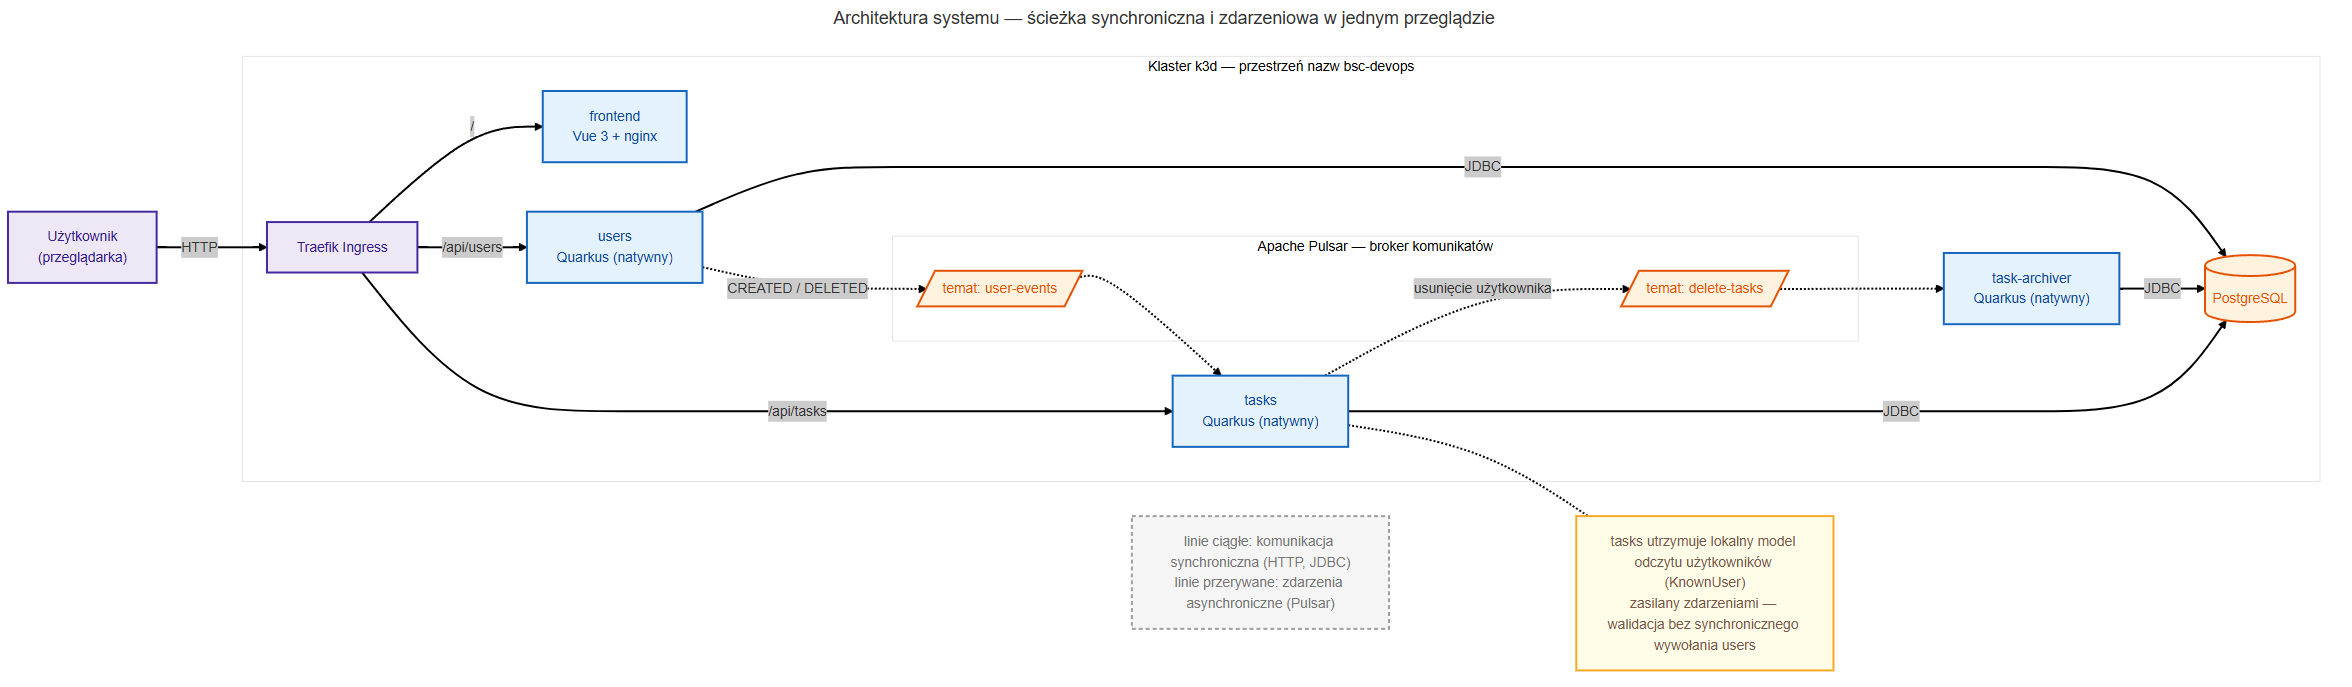
\includegraphics[width=0.9\textwidth]{img/diagrams/02-architektura/architektura-01-system-overview.png}
    \caption{Architektura systemu --- ścieżka synchroniczna (HTTP, JDBC) i~zdarzeniowa (tematy Apache Pulsar) w~jednym przeglądzie (opracowanie własne).}
    \label{fig:system-overview}
\end{figure}

W~warstwie technologicznej zdecydowano się na wykorzystanie ekosystemu Java z~frameworkiem \textit{Quarkus} (ADR-0003). 
Wybór ten podyktowany był charakterem środowiska uruchomieniowego, jakim jest Kubernetes. 
Quarkus, będący rozwiązaniem \textit{Kubernetes-native}, pozwala na znaczną optymalizację zużycia zasobów (pamięci RAM i~procesora) oraz skrócenie czasu uruchamiania aplikacji dzięki kompilacji z~wyprzedzeniem (ang. \textit{Ahead-of-Time}, AOT).
Jest to kluczowe w~architekturze mikroserwisowej, gdzie efektywność kosztowa i~szybkość skalowania są priorytetem.
Aplikacja została zaprojektowana zgodnie z~wytycznymi \textit{Twelve-Factor App}, co zapewnia jej pełną przenośność.

Głównym środowiskiem uruchomieniowym wykorzystywanym w~części praktycznej jest lokalny klaster Kubernetes (\textit{k3d}, ADR-0015).
Takie podejście pozwala na pełną odtwarzalność środowiska produkcyjnego na maszynie deweloperskiej, co jest zgodne z~ideą \textit{Cloud Native}.
Mimo skupienia na środowisku lokalnym, wszystkie zastosowane narzędzia i~konfiguracje (np. Helm, manifesty Kubernetes, aplikacje ArgoCD) są projektowane w~sposób \textit{cloud-agnostic}, umożliwiający ich przeniesienie do publicznych dostawców chmurowych (np. AWS).

\subsection{Struktura części praktycznej}
Opis części praktycznej został ustrukturyzowany w~sposób odzwierciedlający klasyczną pętlę cyklu życia oprogramowania (ang. \textit{DevOps Lifecycle}).
Każdy z~etapów pętli --- od planowania po monitorowanie --- został szczegółowo omówiony w~kontekście wybranych narzędzi i~metodyk.

Przyjęto formę opisu opartą na tzw. „kartach narzędzi”. Dla każdego z~kluczowych komponentów infrastruktury przedstawiono:
\begin{itemize}
    \item opis i~uzasadnienie wyboru danego rozwiązania (często poparte dokumentami ADR),
    \item fragmenty konfiguracji (\textit{Infrastructure as Code}, manifesty YAML, definicje procesów CI/CD),
    \item rolę narzędzia w~całym ekosystemie oraz dobre praktyki inżynierskie zastosowane przy jego konfiguracji.
\end{itemize}

Dzięki takiej strukturze można łatwo zrozumieć, jak poszczególne narzędzia współgrają ze sobą w~ramach kompleksowego procesu dostarczania oprogramowania, a~także jakie decyzje architektoniczne i~inżynierskie stoją za ich implementacją.

Poniższe sekcje szczegółowo opisują realizację kolejnych etapów pętli DevOps.

\subsection{Etap Plan}
Faza planowania (\textit{Plan}) odpowiada za zdefiniowanie wymagań, priorytetyzację zadań i organizację pracy. W niniejszym projekcie etap ten realizowany jest z użyciem platformy Jira jako centrum zarządzania backlogiem.

\subsubsection{Zarządzanie projektami: Jira}
Do zarządzania wymaganiami i planowania prac wykorzystano platformę \textbf{Jira} (projekt \textit{INZ}). Narzędzie to wybrano, ponieważ jest standardem rynkowym i oferuje zaawansowane możliwości obsługi metodyk zwinnych (Agile).

\textbf{Metodyka:}
Agile to rodzina iteracyjnych metodyk wytwarzania oprogramowania, kładących nacisk na częste dostarczanie wartości i adaptację do zmian. Sprinty są podstawową jednostką iteracji w Agile — to ograniczone czasowo okresy pracy (zazwyczaj 1--4 tygodnie), po których dostarcza się działający przyrost produktu. Tablica Kanban to uproszczona alternatywa skupiona na wizualizacji przepływu zadań i ograniczaniu pracy w toku, bez sztywnych iteracji czasowych.

Ponieważ projekt realizowany jest indywidualnie i w ograniczonym czasie, zadania podzielono logicznie na sprinty zgodnie z etapami pętli DevOps, lecz do bieżącego śledzenia pracy zastosowano tablicę Kanban — bardziej odpowiednią dla małych, jednoosobowych projektów.

\textbf{Struktura backlogu:}
Backlog projektu odwzorowuje etapy pętli DevOps. Zdefiniowano pięć Epics odpowiadających sprintom implementacyjnym: \textit{Build}, \textit{Release}, \textit{Deploy}, \textit{Monitor} i \textit{Polish}. W ramach każdego Epica utworzono zestaw zadań (\textit{Tasks}) pokrywających zarówno dostarczenie kodu infrastruktury, jak i uzupełnienie odpowiednich sekcji pracy inżynierskiej. Łącznie backlog liczy 29 zadań.

\textbf{Integracja i dobre praktyki:}
Zastosowano integrację z systemem kontroli wersji GitHub. Każda gałąź kodu (\textit{branch}) jest nazwana według schematu \texttt{feature/INZ-XX-opis}, a wiadomości zatwierdzeń zawierają identyfikator zadania (np. \texttt{feat(helm): INZ-9 create umbrella chart}). Dzięki temu zmiany w kodzie są automatycznie powiązane z odpowiednim zgłoszeniem w Jira, co zapewnia pełną identyfikowalność — od wymagania po konkretną linię kodu.

\begin{figure}[H]
    \centering
    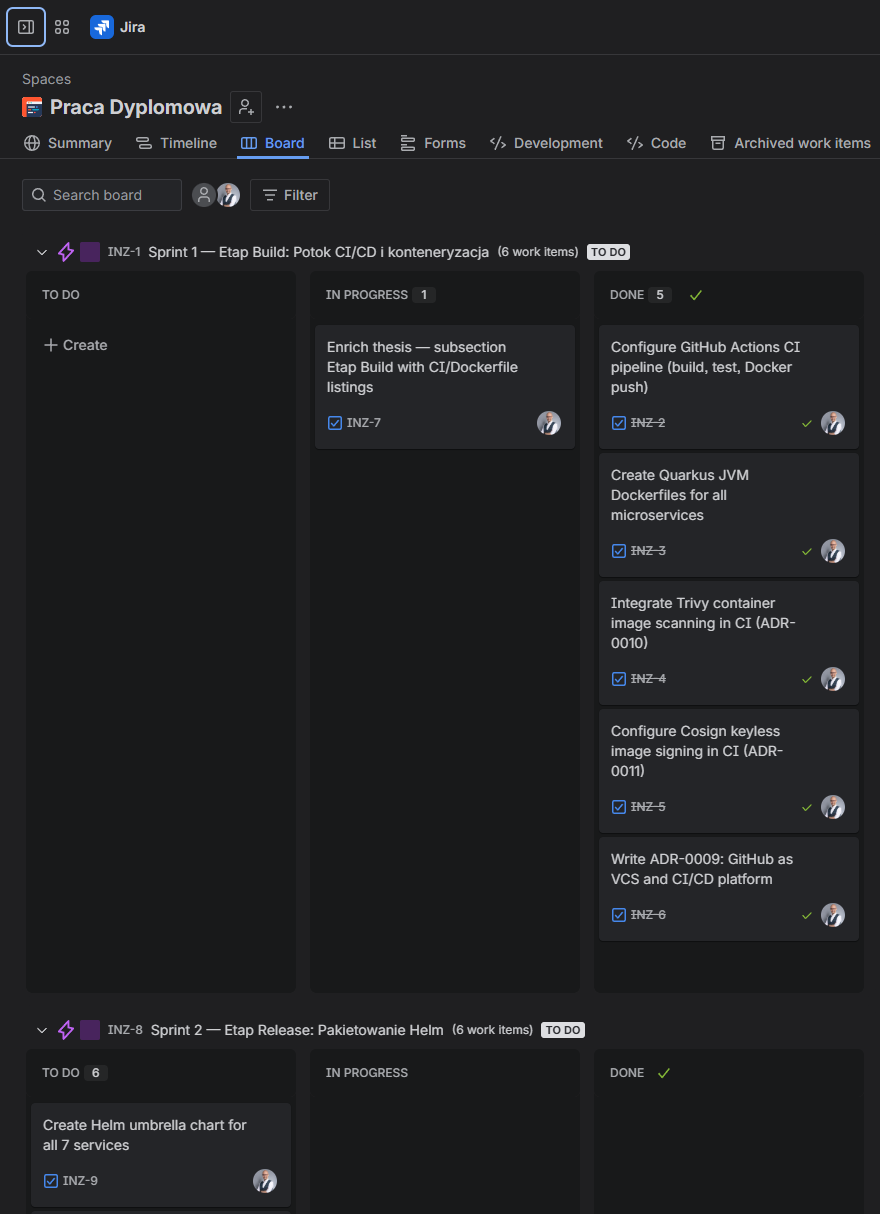
\includegraphics[width=0.75\textwidth]{jira.png}
    \caption{Tablica Kanban projektu INZ w Jira -- widok sprintów i zadań}
    \label{fig:jira-board}
\end{figure}

\subsection{Etap Code}
Faza wytwarzania (\textit{Code}) obejmuje implementację wymagań przy zachowaniu standardów jakości kodu i~spójności historii zmian. Fundamentem tego etapu jest rozproszony system kontroli wersji Git, a~konwencje nazewnictwa zatwierdzeń są wymuszane na poziomie procesu CI.

Proces kodowania realizowany jest przy użyciu nowoczesnych środowisk programistycznych (\textit{IntelliJ IDEA}, \textit{VS Code}), a~sama implementacja opiera się na technologiach realizujących paradygmat mikroserwisów.

Wszystkie komponenty systemu są projektowane zgodnie z~zasadami \textit{Twelve-Factor App}. Kluczowe aspekty to:
\begin{itemize}
    \item \textbf{Konfiguracja:} Cała konfiguracja specyficzna dla środowiska jest wstrzykiwana przez zmienne środowiskowe, a~nie zapisana na stałe w~kodzie.
    \item \textbf{Procesy:} Aplikacje są bezstanowe (ang. \textit{stateless}), co umożliwia ich łatwe skalowanie w~poziomie wewnątrz klastra Kubernetes.
    \item \textbf{Logi:} Są traktowane jako strumień zdarzeń wysyłany na standardowe wyjście, co umożliwia ich centralizację przez narzędzia obserwowalności.
\end{itemize}


\subsubsection{Backend (Java + Quarkus + Native Image)}
Mikroserwisy backendowe zbudowano z~użyciem frameworka \textit{Quarkus} i~skompilowano do natywnych plików wykonywalnych za pomocą \textit{GraalVM Native Image} (kompilacja \textit{Ahead-of-Time}, AOT). W~trybie natywnym Quarkus analizuje ścieżki wykonania kodu w~czasie kompilacji i~wyklucza nieużywane klasy, co skutkuje:
\begin{itemize}
    \item \textbf{Błyskawicznym startem} --- aplikacja jest gotowa do obsługi żądań w~czasie poniżej 100 ms, co skraca czas wznowienia po awarii i~przyspiesza skalowanie poziome w~Kubernetes.
    \item \textbf{Niskim zużyciem pamięci} --- brak środowiska uruchomieniowego JVM zmniejsza ślad pamięciowy kontenera, co bezpośrednio przekłada się na efektywność kosztową w~środowiskach chmurowych.
    \item \textbf{Minimalnym obrazem kontenera} --- obraz oparty na \texttt{ubi-minimal} zawiera wyłącznie system operacyjny i~skompilowany plik binarny, bez JDK ani bibliotek środowiska uruchomieniowego.
\end{itemize}
Wstrzykiwanie zależności realizowane jest przez mechanizm CDI Quarkusa (\textit{ArC}), który w~trybie AOT przetwarza wszystkie adnotacje w~czasie kompilacji, a~nie w~czasie uruchomienia.

\begin{techcard}{Quarkus}

\textbf{Opis:} Quarkus to nowoczesny stos technologiczny Java, określany jako \textit{Supersonic Subatomic Java}. Zaprojektowany z~myślą o~środowiskach \textit{Cloud Native} i~kontenerach, charakteryzuje się bardzo niskim zużyciem pamięci i~błyskawicznym czasem uruchamiania, co jest kluczowe w~architekturze mikrousługowej.

\textbf{Dobre nawyki:}
\begin{itemize}
  \item \textbf{Testowanie natywne (\texttt{@QuarkusIntegrationTest}):} Testy w~trybie natywnym weryfikują, czy optymalizacje AOT nie usunęły elementów wymaganych przez refleksję.
  \item \textbf{Dev Services:} Automatyczne uruchamianie baz danych i~brokerów w~kontenerach podczas prac programistycznych zapewnia spójność środowisk u~wszystkich programistów.
  \item \textbf{Umiar w~refleksji:} Należy preferować rozwiązania obsługujące indeksowanie Jandex i~unikać bibliotek intensywnie korzystających z~dynamicznego ładowania klas.
  \item \textbf{Continuous Testing:} Tryb ciągłego testowania w~konsoli zapewnia natychmiastową informację zwrotną podczas pisania kodu.
\end{itemize}

\textbf{Rola w~projekcie:} Quarkus służy do budowy wydajnych mikroserwisów o~wysokiej gęstości upakowania w~klastrze Kubernetes. Aplikacje zużywają minimalną ilość zasobów, co przekłada się na niższe koszty infrastruktury. Konfigurację aplikacji prezentuje listing \ref{lst:quarkus-app-properties}, a~konfigurację natywnego buildu w~Gradle --- listing \ref{lst:quarkus-native-build} (etap Build).

\end{techcard}

\begin{lstlisting}[caption={Fragment konfiguracji aplikacji (apps/users/src/main/resources/application.properties)}, label={lst:quarkus-app-properties}]
quarkus.application.name=users
quarkus.http.port=8080

quarkus.datasource.db-kind=postgresql
quarkus.hibernate-orm.schema-management.strategy=update

mp.messaging.outgoing.user-events.connector=smallrye-pulsar
mp.messaging.outgoing.user-events.topic=persistent://public/default/user-events
\end{lstlisting}

Zwraca uwagę brak jawnych danych uwierzytelniających w~pliku konfiguracyjnym: w~środowisku deweloperskim ich nieobecność aktywuje mechanizm Dev Services, który automatycznie uruchamia bazę PostgreSQL w~kontenerze, natomiast w~klastrze Kubernetes dane te wstrzykiwane są przez zmienne środowiskowe, zgodnie z~zasadami \textit{Twelve-Factor App}.


\subsubsection{Frontend (Vue 3 + Vite)}
Zgodnie z~decyzją \textit{ADR-0014}, warstwę prezentacji zbudowano z~użyciem frameworka \textit{Vue 3} i~narzędzia budującego \textit{Vite}. Kod pisany jest w~\textit{TypeScript}, a~poprawność typów weryfikuje \textit{vue-tsc} przed każdym buildem produkcyjnym. Komponenty interfejsu komunikują się z~mikroserwisami backendowymi przez REST API.

\begin{techcard}{Vue~3}

\textbf{Opis:} Vue~3 to progresywny framework JavaScript do budowania interfejsów użytkownika. Wprowadza \textit{Composition API} --- umożliwiające organizowanie logiki komponentu według funkcjonalności. Projekt kompilowany jest narzędziem Vite, które wykorzystuje natywne moduły ES podczas prac programistycznych i~Rollup podczas produkcyjnego budowania.

\textbf{Dobre nawyki:}
\begin{itemize}
  \item \textbf{TypeScript przez \texttt{vue-tsc}:} Weryfikacja typów w~komponentach \texttt{.vue} przed buildem produkcyjnym bez generowania plików wyjściowych.
  \item \textbf{Proxy Vite:} Transparentne przekierowanie zapytań do \texttt{/api} na serwer backendowy eliminuje potrzebę konfigurowania CORS w~środowisku deweloperskim.
  \item \textbf{Multi-stage w~Dockerze:} Etap \texttt{npm ci \&\& vite build} produkuje statyczne pliki; obraz docelowy zawiera wyłącznie \texttt{nginx} bez środowiska Node.js.
\end{itemize}

\textbf{Rola w~projekcie:} Vue~3 pełni rolę cienkiej warstwy prezentacji (ang. \textit{thin client}) nad REST API mikroserwisów. Warstwa frontendowa wdrażana jest jako osobny mikroserwis w~Kubernetes z~własnym procesem CI/CD, analogicznie do serwisów backendowych.

\end{techcard}

\begin{lstlisting}[caption={Fragment konfiguracji Vite z~proxy dla środowiska deweloperskiego (apps/frontend/vite.config.ts)}, label={lst:vite-config}]
import { defineConfig } from 'vitest/config';
import vue from '@vitejs/plugin-vue';

export default defineConfig({
  plugins: [vue()],
  server: {
    proxy: {
      '/api/users': {
        target: 'http://localhost:8080',
        rewrite: (path) => path.replace(/^\/api\/users/, '/users'),
      },
      '/api/tasks': {
        target: 'http://localhost:8080',
        rewrite: (path) => path.replace(/^\/api\/tasks/, ''),
      },
    },
  },
});
\end{lstlisting}


\subsubsection{System kontroli wersji: GitHub}
Jako system kontroli wersji i~platformę współpracy wybrano \textbf{GitHub}, oparty na rozproszonym systemie Git. Jest on jedynym źródłem prawdy (ang. \textit{single source of truth}) dla całego monorepozytorium.

\textbf{Standard Conventional Commits:}
Zgodnie z~decyzją projektową \textit{ADR-0004}, wprowadzono standard \textbf{Conventional Commits}. Polega on na nadawaniu opisom zatwierdzeń ustrukturyzowanej formy (np. \texttt{feat:}, \texttt{fix:}, \texttt{chore:}) \cite{conventionalCommits}.
\begin{itemize}
    \item \textbf{Uzasadnienie:} Standaryzacja pozwala na automatyczne generowanie list zmian (ang. \textit{changelogs}) oraz automatyzację wersjonowania semantycznego (ang. \textit{Semantic Versioning}).
    \item \textbf{Rola w~CI/CD:} Czytelna historia zmian umożliwia narzędziom automatyzującym precyzyjne określenie, które komponenty systemu wymagają przebudowania i~wdrożenia po każdej zmianie w~monorepozytorium.
\end{itemize}

Poniższy przykład ilustruje kompletny opis zatwierdzenia zgodny ze standardem. Nagłówek zawiera typ, zakres oraz zwięzły opis zmiany, a~stopka (ang. \textit{footer}) powiązuje commit z~konkretnym zadaniem w~systemie Jira:

\begin{lstlisting}[caption={Przykład opisu zatwierdzenia zgodnego ze standardem Conventional Commits}, label={lst:conventional-commit}]
feat(helm): create umbrella chart for all 7 services

Aggregates all microservice charts under a single parent
chart, enabling one-command deployment of the full stack.

Resolves: INZ-9
\end{lstlisting}


\subsection{Etap Build}
Faza budowania (\textit{Build}) odpowiada za przekształcenie kodu źródłowego w~gotowe do wdrożenia artefakty. W~architekturze \textit{Cloud Native} proces ten kończy się wytworzeniem obrazu kontenera.

\subsubsection{Orkiestracja procesu CI/CD: GitHub Actions}
Zgodnie z~decyzją \textit{ADR-0009}, jako platformę CI/CD wybrano \textbf{GitHub Actions}. Pozwala ona na definiowanie procesów CI/CD w~formie kodu YAML bezpośrednio w~repozytorium, co jest zgodne z~zasadą \textit{Everything as Code} i~eliminuje potrzebę utrzymywania zewnętrznego serwera CI.

\textbf{Rola w~projekcie:}
GitHub Actions pełni funkcję silnika CI (\textit{Continuous Integration}), który reaguje na zdarzenia w~repozytorium (np. \textit{pull request} lub \textit{push} do gałęzi głównej). Proces CI/CD automatycznie uruchamia kompilację, testy oraz budowanie obrazów, zapewniając szybką pętlę informacji zwrotnej dla programisty.

\textbf{Struktura procesów CI/CD:}
Dla każdego mikroserwisu zdefiniowano oddzielny plik \textit{workflow} (np. \texttt{ci-users.yml}), uruchamiany wyłącznie przy zmianach w~katalogu danego serwisu. Takie podejście eliminuje zbędne uruchomienia procesu CI dla komponentów, których kod nie uległ zmianie.

\begin{lstlisting}[language=yaml, caption={Fragment procesu CI --- budowanie i~push obrazu natywnego (.github/workflows/ci-users.yml)}, label={lst:github-actions-build}]
jobs:
  build:
    name: Build, Test, Scan & Push — users
    runs-on: ubuntu-latest
    permissions:
      contents: read
      id-token: write   # wymagane przez Cosign keyless signing
    steps:
      - uses: actions/checkout@v7
      - name: Set up JDK 25
        uses: actions/setup-java@v5
        with:
          java-version: '25'
          distribution: temurin
          cache: gradle
      - name: Run tests
        run: ./gradlew :apps:users:test --no-daemon
      - name: Build application and container image
        run: |
          ./gradlew :apps:users:imageBuild \
            -Dquarkus.container-image.tag=${{ github.sha }} \
            --no-daemon
\end{lstlisting}

Pełny przebieg procesu CI --- od zdarzenia w~repozytorium, przez testy i~budowanie obrazu natywnego, po bramkę skanowania i~podpis artefaktu --- przedstawia rysunek~\ref{fig:ci-pipeline}. Rysunek~\ref{fig:ci-governance} pokazuje ten sam proces z~perspektywy zdarzeń: bieg dla \textit{pull requesta} jedynie waliduje zmiany, a~dopiero bieg dla gałęzi \texttt{main} publikuje i~podpisuje obraz; ochrona gałęzi blokuje scalenie do czasu pomyślnego zakończenia weryfikacji CI.

\begin{figure}[H]
    \centering
    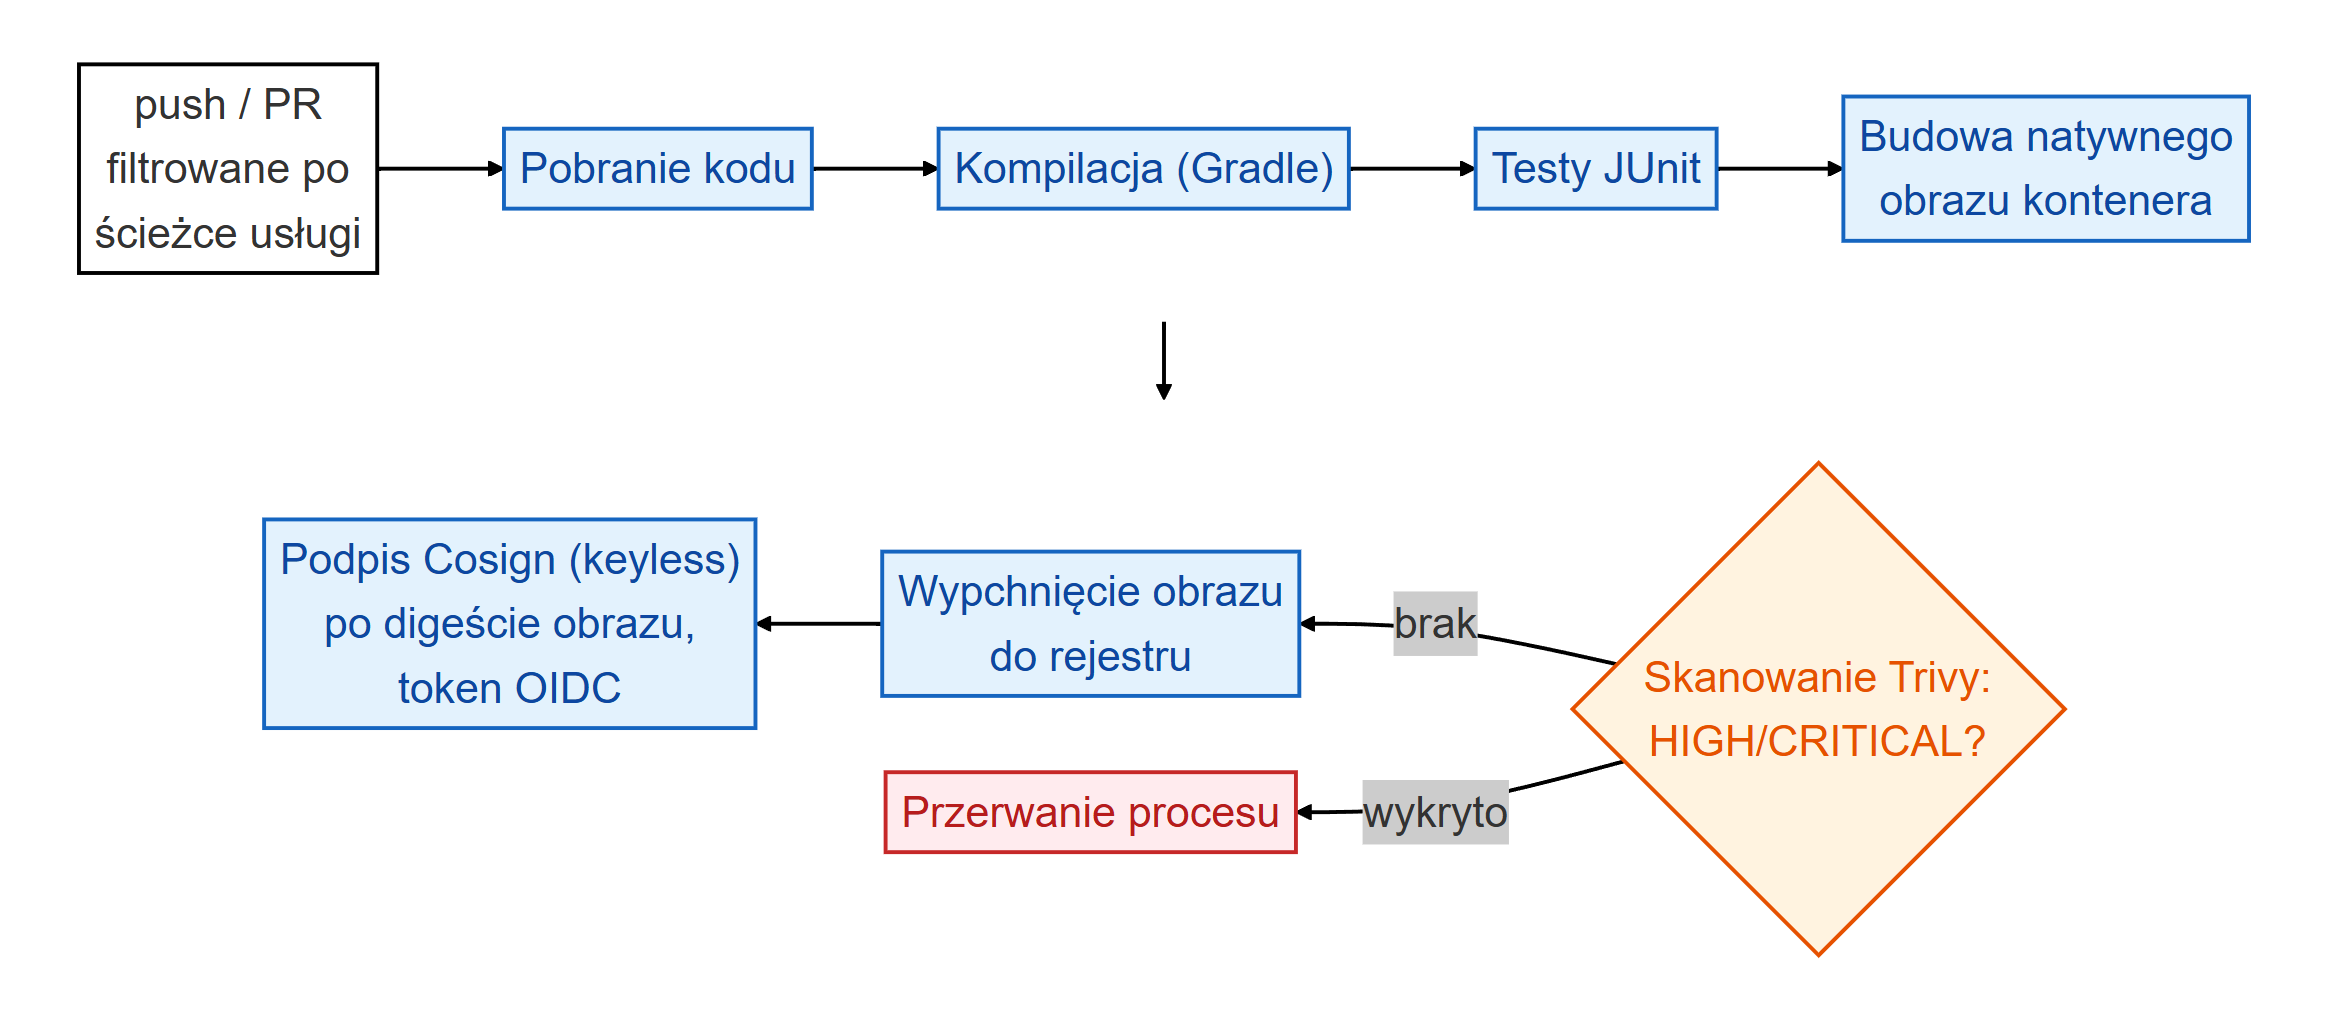
\includegraphics[width=\textwidth]{img/diagrams/04-build/build-01-ci-pipeline.png}
    \caption{Proces CI z~bezpieczeństwem Shift-Left --- skanowanie Trivy jako bramka przed publikacją, podpis Cosign po wypchnięciu obrazu (por.\ rys.~\ref{fig:ci-governance}; opracowanie własne).}
    \label{fig:ci-pipeline}
\end{figure}

\begin{figure}[H]
    \centering
    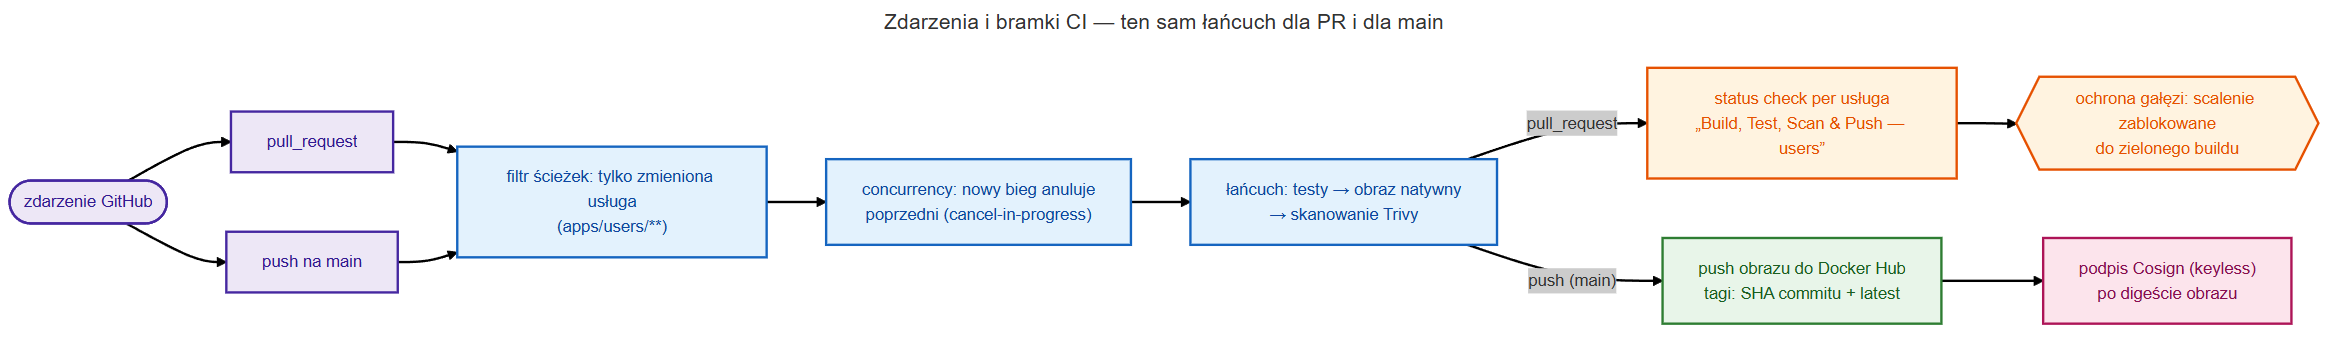
\includegraphics[width=0.6\textwidth]{img/diagrams/04-build/build-02-flow-ci-governance.png}
    \caption{Zdarzenia i~bramki tego samego procesu --- walidacyjny bieg \textit{pull requesta} i~publikujący bieg \texttt{main} z~ochroną gałęzi (por.\ rys.~\ref{fig:ci-pipeline}; opracowanie własne).}
    \label{fig:ci-governance}
\end{figure}

\subsubsection{Budowanie artefaktów: Gradle i~NPM}
W~zależności od komponentu wykorzystywane są wyspecjalizowane narzędzia budujące:
\begin{itemize}
    \item \textbf{Gradle (Backend):} Zarządza zależnościami projektu Java/Quarkus, kompiluje kod oraz uruchamia testy jednostkowe. Wybrano go (ADR-0008) ze względu na elastyczność i~wydajność (mechanizm \textit{build cache}).
    \item \textbf{Vite (Frontend):} Odpowiada za budowanie zoptymalizowanej paczki produkcyjnej aplikacji Vue 3. Vite wykorzystuje natywne moduły ES podczas prac programistycznych, co skraca czas przeładowania do milisekund, a~NPM zarządza zależnościami projektu.
\end{itemize}

\subsubsection{Konteneryzacja: Docker + Dockerfile}
Zgodnie z~decyzją \textit{ADR-0005}, jako standard budowania obrazów wybrano pliki \textbf{Dockerfile}. Wybór ten podyktowany był chęcią zachowania pełnej przejrzystości procesu, co ma kluczowe znaczenie w~pracy inżynierskiej.

\begin{techcard}{Docker}

\textbf{Opis:} Docker to platforma konteneryzacji pozwalająca na pakowanie oprogramowania wraz z~całym środowiskiem uruchomieniowym w~lekkie, przenośne kontenery. Dzięki temu aplikacja działa identycznie niezależnie od maszyny docelowej.

\textbf{Dobre nawyki:}
\begin{itemize}
  \item \textbf{Multi-stage builds:} Oddzielenie środowiska kompilacji od uruchomieniowego redukuje rozmiar końcowego obrazu i~eliminuje narzędzia budujące z~obrazu produkcyjnego.
  \item \textbf{Zasada najniższych uprawnień:} Kontenery nie powinny działać jako użytkownik \texttt{root} --- należy zdefiniować wydzielonego użytkownika technicznego (patrz listing \ref{lst:dockerfile-native}).
  \item \textbf{Precyzyjne tagowanie:} Unikanie tagu \texttt{latest} na rzecz konkretnych wersji (semantycznych lub hashów git) zapewnia powtarzalność wdrożeń.
  \item \textbf{Plik \texttt{.dockerignore}:} Wykluczanie zbędnych plików (np. \texttt{node\_modules}, \texttt{.git}, \texttt{target/}) przyspiesza budowanie i~zapobiega wyciekom danych wrażliwych.
\end{itemize}

\textbf{Rola w~projekcie:} Docker pełni rolę „pakowacza” --- przed jego użyciem dostępny jest skompilowany plik binarny, a~po zbudowaniu obrazu powstaje gotowy do wdrożenia artefakt uruchamialny w~dowolnym środowisku kontenerowym. Dockerfile dla trybu natywnego przedstawia listing \ref{lst:dockerfile-native}.

\end{techcard}

\textbf{Docker i~Quarkus --- kompilacja AOT i~minimalne obrazy:}
Quarkus generuje gotowe pliki \texttt{Dockerfile.native} przeznaczone dla obrazów zbudowanych w~trybie GraalVM \textit{Ahead-of-Time} (AOT). Kompilacja natywna odbywa się wewnątrz kontenera Mandrel (dystrybucja GraalVM zoptymalizowana pod kątem Quarkusa) uruchamianego przez Gradle w~procesie CI, bez konieczności instalowania GraalVM bezpośrednio na maszynie CI. Konfigurację narzędzia budującego zawiera plik \texttt{build.gradle}:

\begin{lstlisting}[language=groovy, caption={Konfiguracja natywnego buildu Quarkusa w~Gradle (apps/users/build.gradle)}, label={lst:quarkus-native-build}]
quarkusBuild {
    nativeArgs {
        containerBuild = true
        builderImage = "quay.io/quarkus/ubi10-quarkus-mandrel-builder-image:jdk-25"
    }
}
\end{lstlisting}

Wynikiem kompilacji jest samodzielny plik wykonywalny (\texttt{build/*-runner}), który nie wymaga środowiska JVM. Dockerfile kopiuje go do minimalnego obrazu bazowego Red Hat UBI:

\begin{lstlisting}[language=docker, caption={Natywny Dockerfile Quarkusa dla mikroserwisu \textit{users} (apps/users/src/main/docker/Dockerfile.native)}, label={lst:dockerfile-native}]
FROM registry.access.redhat.com/ubi10/ubi-minimal:10.2
WORKDIR /work/
RUN chown 1001 /work \
    && chmod "g+rwX" /work \
    && chown 1001:root /work
COPY --chown=1001:root --chmod=0755 build/*-runner /work/application

EXPOSE 8080
USER 1001

ENTRYPOINT ["./application", "-Dquarkus.http.host=0.0.0.0"]
\end{lstlisting}

Obraz końcowy zawiera wyłącznie minimalny system operacyjny i~skompilowany plik binarny aplikacji --- bez JVM, JDK ani żadnych narzędzi budujących. Warstwa frontendowa (\textit{Vue 3}) stosuje klasyczny wzorzec wieloetapowy: etap kompilacji Vite produkujący statyczne pliki w~katalogu \texttt{dist/}, a~następnie serwowanie ich przez minimalny obraz \textit{nginx}.
Całą ścieżkę budowania natywnego --- na tle klasycznej ścieżki JVM --- podsumowuje rysunek~\ref{fig:native-build}: kosztem długiej kompilacji AOT (analiza zamkniętego świata --- założenie, że cały kod potrzebny w~czasie działania jest znany w~chwili kompilacji) uzyskuje się start w~milisekundach oraz minimalny obraz pozbawiony środowiska JVM.

\begin{figure}[H]
    \centering
    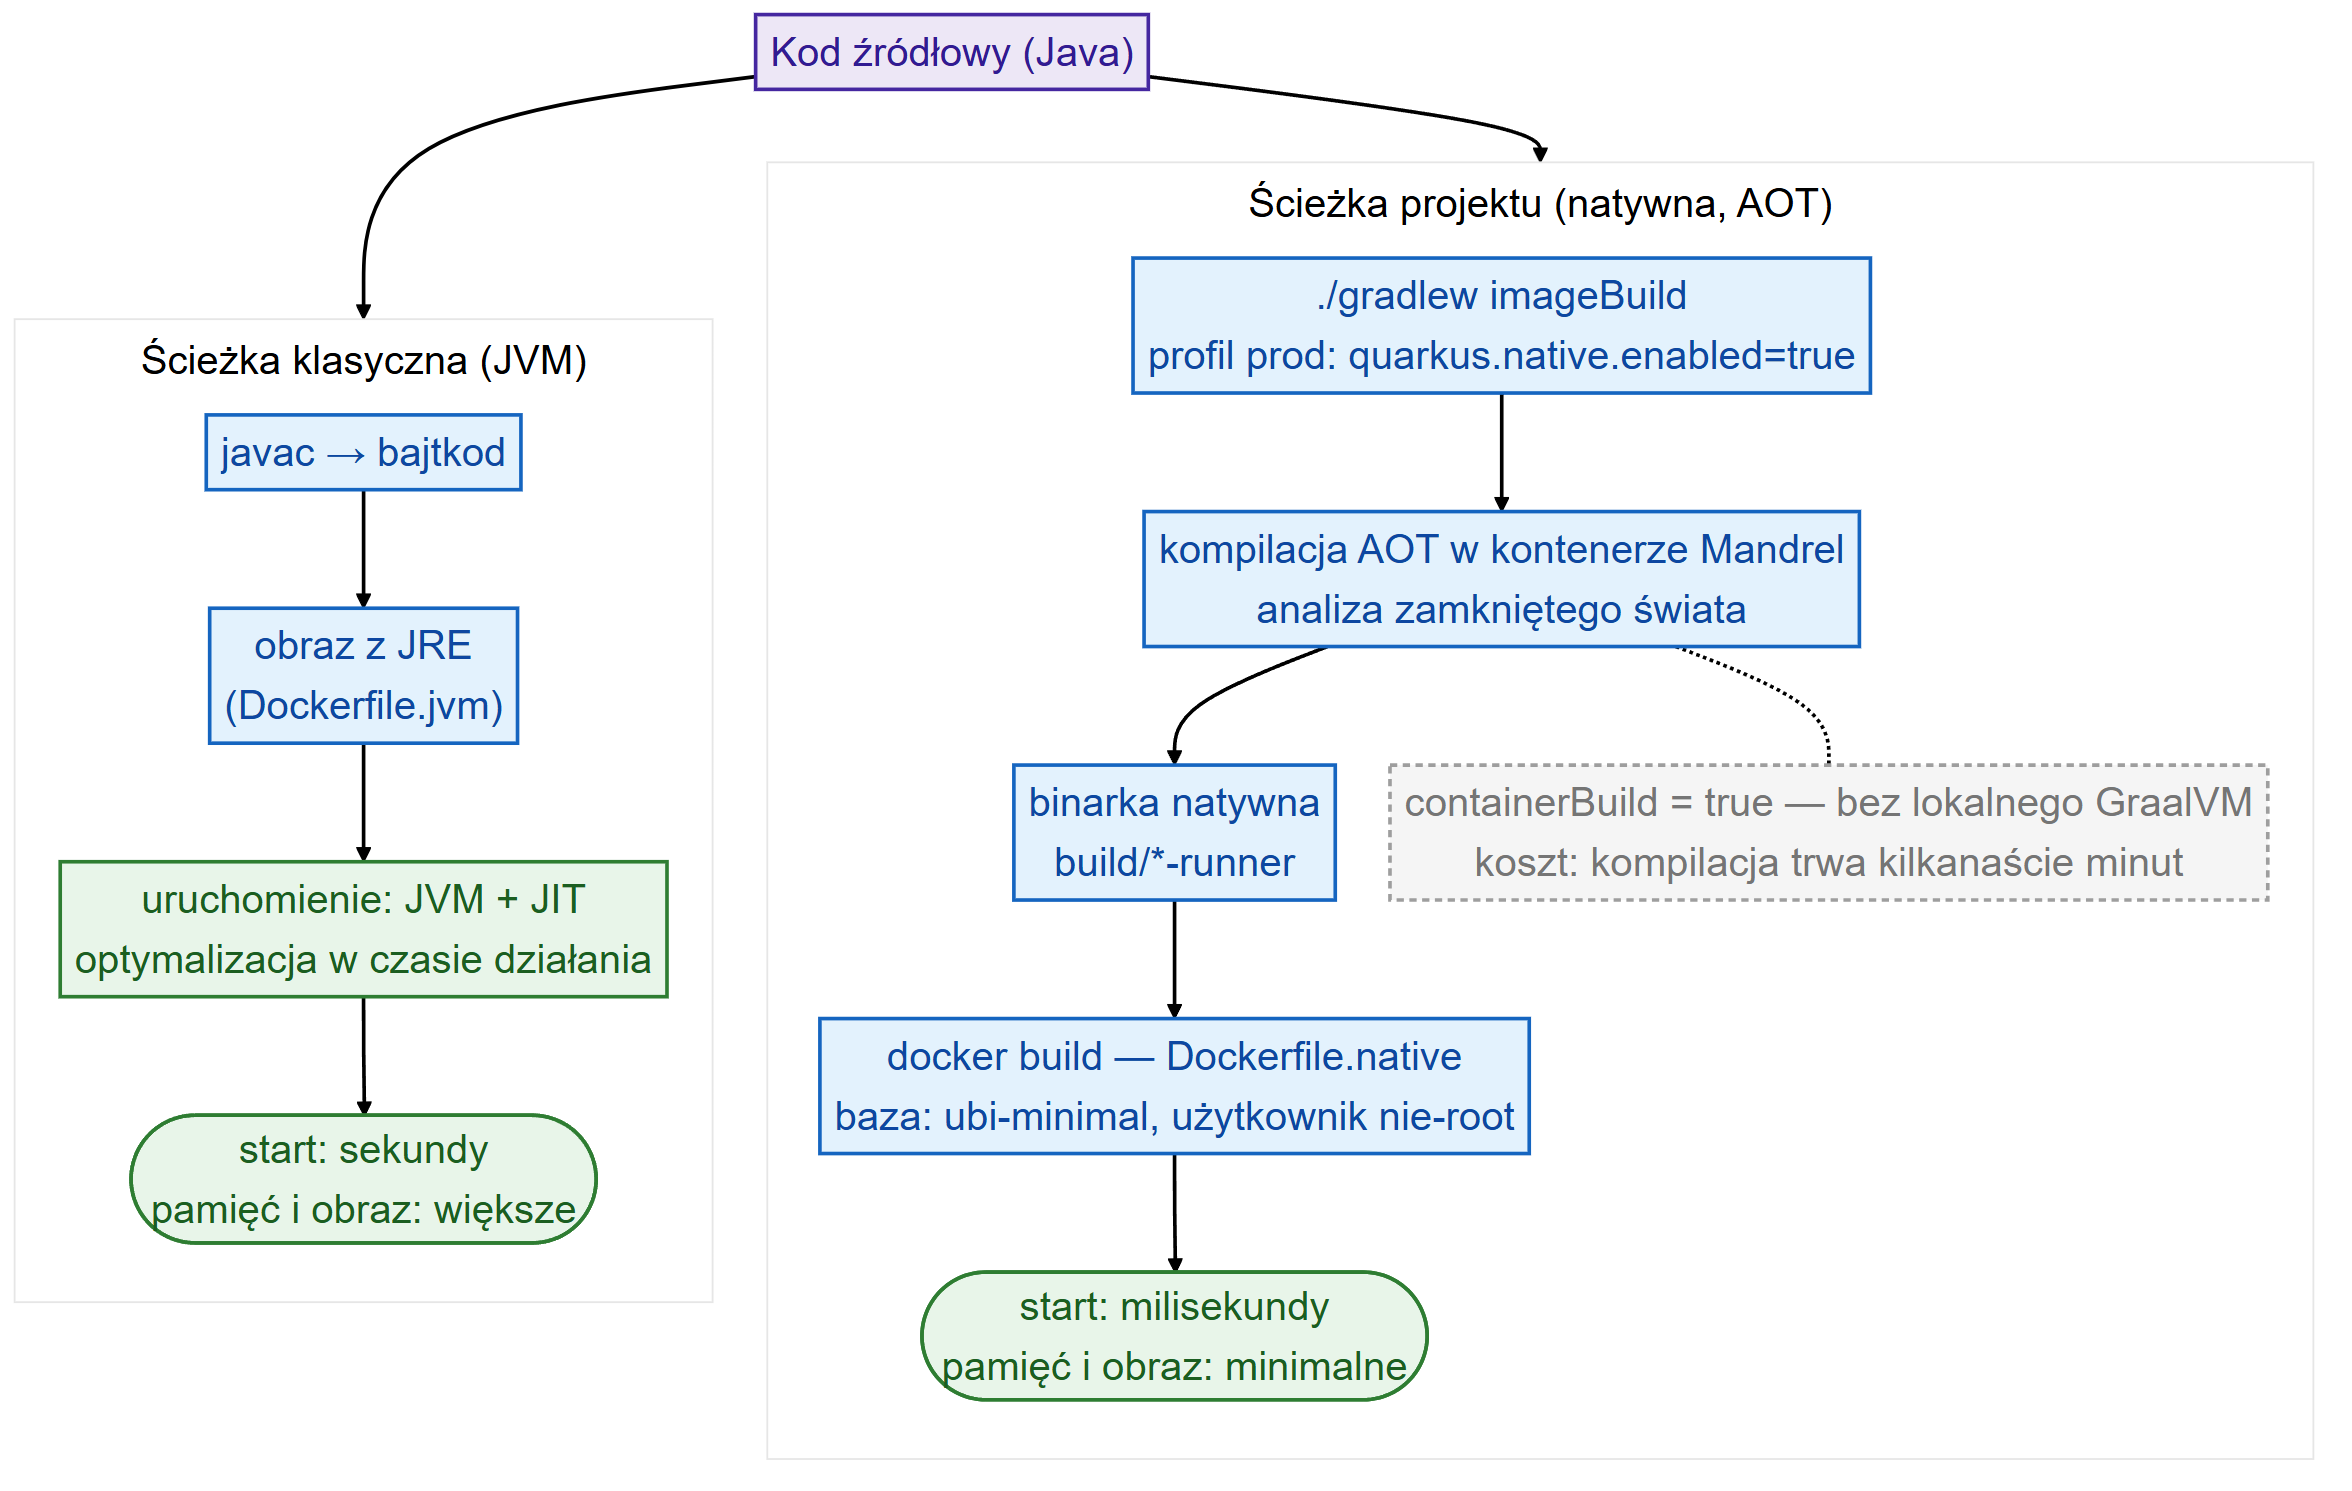
\includegraphics[width=\textwidth]{img/diagrams/04-build/build-03-flow-native-build.png}
    \caption{Anatomia budowania natywnego --- ścieżka klasyczna (JVM, optymalizacja JIT w~czasie działania) na tle ścieżki projektu (kompilacja AOT w~kontenerze Mandrel, minimalny obraz); koszt kompilacji wymieniony na szybki start i~małe zużycie pamięci (opracowanie własne).}
    \label{fig:native-build}
\end{figure}

\textbf{Shift-Left Security:}
Bezpieczeństwo jest weryfikowane już na etapie budowania:
\begin{itemize}
    \item \textbf{Trivy (ADR-0010):} Każdy zbudowany obraz jest skanowany pod kątem znanych podatności (CVE) w~bibliotekach systemowych i~aplikacyjnych.
\begin{lstlisting}[language=yaml, caption={Skanowanie obrazu narzędziem Trivy w~procesie CI (.github/workflows/ci-users.yml)}, label={lst:trivy-scan}]
- name: Scan image with Trivy
  uses: aquasecurity/trivy-action@v0.36.0
  with:
    image-ref: mateuszwas/users:${{ github.sha }}
    format: table
    exit-code: '1'
    ignore-unfixed: true
    vuln-type: os,library
    severity: HIGH,CRITICAL
\end{lstlisting}
    \item \textbf{Cosign (ADR-0011):} Obrazy są cyfrowo podpisywane metodą \textit{keyless signing} (Sigstore), co zapewnia ich integralność i~pozwala na weryfikację pochodzenia artefaktu przed jego uruchomieniem w~klastrze.
\end{itemize}

\subsection{Etap Test}
Automatyzacja testów jest fundamentem zaufania do procesu CI/CD. W projekcie testy są integralną częścią każdego łańcucha budowania i stanowią bramkę blokującą przejście do dalszych, kosztownych etapów.

\subsubsection{Testy integracyjne: JUnit 5 i @QuarkusTest}
Podstawowym narzędziem weryfikacji poprawności logiki biznesowej jest framework \textbf{JUnit 5}, zintegrowany z biblioteką testową Quarkusa poprzez zależność \texttt{quarkus-junit5}.

\textbf{Adnotacja \texttt{@QuarkusTest}:}
W odróżnieniu od klasycznych testów jednostkowych, adnotacja \texttt{@QuarkusTest} uruchamia przed zestawem testów pełny kontekst aplikacji Quarkus -- z kontenerem CDI, warstwą REST i skonfigurowanymi połączeniami do zewnętrznych usług. Testy mogą zatem weryfikować rzeczywiste zachowanie endpointów HTTP przy użyciu zintegrowanej biblioteki \textbf{RestAssured}. Jej API wzoruje się na notacji \textbf{Gherkin} (\textit{Given/When/Then}), stosowanej w metodykach BDD (\textit{Behaviour-Driven Development}): blok \texttt{given()} definiuje warunki wstępne żądania (nagłówki, ciało), \texttt{when()} wykonuje wywołanie HTTP, a \texttt{then()} weryfikuje odpowiedź. Dzięki temu intencja testu jest czytelna bez znajomości samej biblioteki:

\begin{lstlisting}[language=java, caption={Test integracyjny endpointu REST mikroserwisu \textit{users} (apps/users/src/test/.../UserResourceTest.java)}, label={lst:quarkus-test-users}]
@QuarkusTest
class UserResourceTest {

    @Test
    void testListUsers() {
        given()
            .when().get("/users")
            .then()
            .statusCode(200);
    }

    @Test
    void testCreateUser() {
        given()
            .contentType(JSON)
            .body("{\"name\":\"Alice\",\"email\":\"alice@example.com\"}")
            .when().post("/users")
            .then()
            .statusCode(201);
    }
}
\end{lstlisting}

\textbf{Dev Services -- automatyczna infrastruktura testowa:}
Kluczową cechą ekosystemu Quarkusa jest mechanizm \textbf{Dev Services}: jeśli w konfiguracji aplikacji nie podano jawnego adresu URL bazy danych, Quarkus automatycznie uruchamia kontener PostgreSQL przy użyciu biblioteki \textit{Testcontainers}. Programista nie musi konfigurować środowiska testowego ani utrzymywać lokalnej instancji bazy -- wystarczy wywołanie \texttt{./gradlew test}. Testy zawsze działają na izolowanej, świeżej instancji bazy danych, co eliminuje klasyczny problem współdzielonego stanu testowego.

\textbf{Izolacja transakcyjna -- \texttt{@TestTransaction}:}
Dla testów weryfikujących logikę perzystencji stosowana jest adnotacja \texttt{@TestTransaction}: każdy test jest owijany w transakcję bazodanową, która po jego zakończeniu jest automatycznie wycofywana (\textit{rollback}). Zapewnia to pełną izolację między testami bez konieczności ręcznego czyszczenia stanu bazy. Wzorzec ten zastosowano w testach konsumenta zdarzeń mikroserwisu \textit{tasks}:

\begin{lstlisting}[language=java, caption={Test konsumenta zdarzeń z izolacją @TestTransaction (apps/tasks/src/test/.../UserEventConsumerTest.java)}, label={lst:test-transaction}]
@QuarkusTest
class UserEventConsumerTest {

    @Inject
    UserEventConsumer consumer;

    @Test
    @TestTransaction
    void createdEventPersistsKnownUser() {
        consumer.consume(new UserEvent(99L, UserEvent.Type.CREATED));
        assertNotNull(KnownUser.findById(99L));
    }

    @Test
    @TestTransaction
    void deletedEventRemovesKnownUser() {
        KnownUser u = new KnownUser();
        u.id = 42L;
        KnownUser.persist(u);

        consumer.consume(new UserEvent(42L, UserEvent.Type.DELETED));
        assertNull(KnownUser.findById(42L));
    }
}
\end{lstlisting}

\subsubsection{Testy jako bramka w łańcuchu CI/CD}
Użycie testów w łańcuchu CI na początku jest celowe i ma bezpośredni wpływ na efektywność procesu (listing~\ref{lst:github-actions-build}). Krok \texttt{Run tests} poprzedza budowanie natywnego obrazu kontenera (\texttt{imageBuild}), które korzysta z kompilatora GraalVM AOT i trwa kilkanaście minut. Niepowodzenie testu natychmiast przerywa łańcuch -- bez zbędnego zużycia zasobów CI na kosztowną kompilację natywną.

\begin{itemize}
    \item \textbf{Zakres:} Testy pokrywają kluczowe komponenty domeny (logika REST, perzystencja przez Panache) oraz integrację z bazą danych uruchamianą przez Dev Services, bez konieczności mocków.
    \item \textbf{Anulowanie przestarzałych uruchomień:} Konfiguracja w sekcji \texttt{concurrency} z ustawieniem \texttt{cancel-in-progress: true} gwarantuje, że nowe uruchomienie łańcucha dla tej samej gałęzi automatycznie anuluje poprzednie, wciąż aktywne uruchomienie. Eliminuje to sytuacje, w których wyniki przestarzałych łańcuchów blokują lub dezorientują recenzentów kodu.
    \item \textbf{Izolacja per serwis:} Każdy mikroserwis posiada oddzielny plik workflow uruchamiany wyłącznie przy zmianach w jego katalogu. Testy serwisu \textit{users} nie są uruchamiane przy zmianie kodu \textit{tasks} -- co skraca czas informacji zwrotnej i obniża koszty CI.
\end{itemize}

\subsubsection{Widoczność wyników w procesie Pull Request}
GitHub Actions raportuje wyniki każdego zadania (\textit{job}) jako \textbf{status check} bezpośrednio w widoku Pull Requesta. Zadanie \texttt{Build, Test, Scan \& Push} dla każdego serwisu widoczne jest jako oddzielny, nazwany check -- programista natychmiast identyfikuje, który z mikroserwisów jest \textit{czerwony} i z jakiego powodu. Dopóki wszystkie aktywowane łańcuchy nie zakończą się sukcesem, scalenie PR jest zablokowane, co egzekwuje zasadę \textit{green build before merge} bez konieczności ręcznej interwencji recenzenta.

\subsection{Etap Release}
Faza wydania (\textit{Release}) koncentruje się na bezpiecznym przechowywaniu artefaktów oraz ich wersji, gotowych do wdrożenia w~środowiskach docelowych.

\subsubsection{Rejestr obrazów: Docker Hub}
Jako centralne repozytorium obrazów kontenerowych wykorzystano platformę \textbf{Docker Hub}.
\begin{itemize}
    \item \textbf{Rola w~projekcie:} Po pomyślnym zakończeniu etapu budowania i~testowania, obrazy mikroserwisów są wysyłane (ang. \textit{push}) do prywatnych lub publicznych repozytoriów w~Docker Hub. Każdy obraz jest oznaczony unikalnym tagiem (np. skrótem \textit{commit SHA} lub numerem wersji semantycznej), co zapewnia pełną identyfikowalność.
    \item \textbf{Uzasadnienie:} Docker Hub jest natywnie obsługiwany przez większość narzędzi CI/CD oraz klastry Kubernetes, co upraszcza proces pobierania obrazów podczas wdrożenia.
\end{itemize}

\subsubsection{Pakietowanie dla Kubernetes: Helm}
Zarządzanie manifestami YAML dla wielu mikroserwisów staje się trudne bez odpowiedniego narzędzia. Zgodnie z~decyzją \textit{ADR-0012}, jako standard pakietowania dla Kubernetes wybrano \textbf{Helm} — menedżer pakietów pozwalający na szablonowanie i~wersjonowanie konfiguracji infrastruktury.

\begin{techcard}{Helm}

\textbf{Opis:} Helm to menedżer pakietów dla Kubernetes, analogiczny do \texttt{apt} czy \texttt{brew} w~świecie systemów operacyjnych. Pozwala na definiowanie, instalowanie i~aktualizowanie złożonych aplikacji Kubernetes jako pojedynczych, wersjonowanych pakietów zwanych \textbf{chartami}. Chart to zestaw szablonów YAML sparametryzowanych wartościami z~pliku \texttt{values.yaml}. Helm śledzi historię wdrożeń jako kolejne rewizje, co umożliwia natychmiastowy rollback.

\textbf{Dobre nawyki:}
\begin{itemize}
  \item \textbf{Umbrella chart:} Grupowanie powiązanych mikroserwisów w~jeden chart pozwala wdrożyć cały stos jednym poleceniem \texttt{helm install}, zachowując spójność wersji wszystkich komponentów.
  \item \textbf{Parametryzacja przez values:} Wartości specyficzne dla środowiska (tagi obrazów, liczba replik, limity zasobów) powinny być wydzielone do osobnych plików \texttt{values-prod.yaml}, a~nie zakodowane na sztywno w~szablonach.
  \item \textbf{Wersjonowanie wydań (ang. \textit{releases}):} Każda zmiana wprowadzona przez \texttt{helm upgrade} tworzy nową rewizję. Polecenie \texttt{helm rollback} natychmiast przywraca poprzedni stan klastra bez ręcznej edycji manifestów.
  \item \textbf{Helpery szablonów (\texttt{\_helpers.tpl}):} Wspólne etykiety i~selektory należy definiować jako nazwane szablony w~\texttt{\_helpers.tpl}, aby zapewnić spójność i~uniknąć powielania kodu YAML.
\end{itemize}

\textbf{Rola w~projekcie:} Helm pełni rolę menedżera infrastruktury projektu. Umbrella chart \texttt{bsc-devops} opisuje wszystkie komponenty stosu w~jednym, wersjonowanym pakiecie.

\end{techcard}

\textbf{Umbrella chart i~parametryzacja środowisk:}
W~projekcie zastosowano wzorzec \textbf{umbrella chart}: jeden chart \texttt{bsc-devops} obejmuje wszystkie sześć komponentów stosu (serwisy \textit{users}, \textit{tasks}, \textit{task-archiver}, \textit{frontend}, bazę PostgreSQL oraz broker Pulsar). Każdy komponent może być niezależnie włączony lub wyłączony flagą \texttt{enabled}. Konfiguracja zasobów obliczeniowych i~tagów obrazów jest wydzielona do \texttt{values.yaml}:

\begin{lstlisting}[language=yaml, caption={Fragment \texttt{values.yaml} umbrella chartu --- parametryzacja serwisu \textit{users} (infrastructure/helm/bsc-devops/values.yaml)}, label={lst:helm-values}]
users:
  enabled: true
  image:
    repository: "docker.io/mateuszwas/users"
    tag: "1.2.0"
  replicas: 1
  resources:
    requests:
      cpu: "50m"
      memory: "64Mi"
    limits:
      cpu: "500m"
      memory: "256Mi"
\end{lstlisting}

\textbf{Szablony Go i~helpery:}
Szablony Helm korzystają z~silnika Go \texttt{text/template}. Wyrażenia \texttt{\{\{ include \}\}} wywołują nazwane helpery zdefiniowane w~pliku \texttt{\_helpers.tpl}. Przykładowo, helper \texttt{bsc-devops.imageRef} scala repozytorium z~tagiem obrazu, a~globalny tag może nadpisywać wartość per-serwis:

\begin{lstlisting}[language=yaml, caption={Fragment szablonu Deployment serwisu \textit{users} z~interpolacją wartości (infrastructure/helm/bsc-devops/templates/users.yaml)}, label={lst:helm-template}]
spec:
  replicas: {{ .Values.users.replicas }}
  template:
    spec:
      containers:
        - name: users
          image: {{ include "bsc-devops.imageRef"
            (dict "repo" .Values.users.image.repository
                  "tag"  .Values.users.image.tag
                  "ctx"  .) }}
          resources:
            {{- toYaml .Values.users.resources | nindent 12 }}
          livenessProbe:
            tcpSocket:
              port: 8080
            initialDelaySeconds: 10
            periodSeconds: 20
\end{lstlisting}

\subsubsection{Dystrybucja chartu: GitHub Container Registry}
Gotowy chart Helm jest publikowany jako artefakt OCI w~rejestrze \textbf{GitHub Container Registry} (GHCR). Dzięki natywnej obsłudze formatu OCI w~Helm 3.8+ możliwe jest traktowanie rejestru kontenerów jako uniwersalnego magazynu artefaktów --- bez potrzeby utrzymywania zewnętrznych repozytoriów chartów (np. ChartMuseum).

\textbf{Uzasadnienie wyboru GHCR:}
\begin{itemize}
    \item \textbf{Brak zewnętrznych zależności:} GHCR jest integralną częścią GitHub --- nie wymaga dodatkowych usług ani konfiguracji.
    \item \textbf{Jednolite logowanie:} Uwierzytelnianie odbywa się przez \texttt{GITHUB\_TOKEN} z~uprawnieniem \texttt{packages:write}, ten sam mechanizm co w~przypadku obrazów Docker.
    \item \textbf{Wersjonowanie OCI:} Tag artefaktu odpowiada wersji semantycznej chartu z~\texttt{Chart.yaml}, co zapewnia pełną identyfikowalność.
\end{itemize}

\textbf{Dwuetapowy proces publikacji:}
Dystrybucja chartu realizowana jest przez dwa oddzielne procesy CI/CD, powiązane zdarzeniem utworzenia tagu git. Podejście to rozdziela walidację od publikacji:

\begin{lstlisting}[language=yaml, caption={Proces CD publikujący chart do GHCR (.github/workflows/cd-helm.yml)}, label={lst:cd-helm}]
on:
  push:
    tags:
      - 'chart-apps-*'

jobs:
  publish:
    permissions:
      contents: read
      packages: write
    steps:
      - uses: actions/checkout@v7
      - uses: azure/setup-helm@v5
      - name: Log in to GHCR
        run: |
          echo "${{ secrets.GITHUB_TOKEN }}" | helm registry login ghcr.io \
            --username ${{ github.actor }} --password-stdin
      - name: Package chart
        run: helm package infrastructure/helm/bsc-devops
      - name: Push chart to GHCR
        run: helm push bsc-devops-apps-*.tgz oci://ghcr.io/${{ github.repository_owner }}/charts
\end{lstlisting}

Proces \texttt{ci-helm} waliduje chart i~--- przy każdym wypchnięciu zmian na gałąź \texttt{main} --- odczytuje wersję z~\texttt{Chart.yaml} i~tworzy tag git \texttt{chart-apps-<wersja>}. Tag ten wyzwala proces \texttt{cd-helm}, który pakuje chart poleceniem \texttt{helm package} i~publikuje artefakt OCI pod adresem \texttt{ghcr.io/mwas-inz/charts/bsc-devops-apps:<wersja>}.

Cały proces --- od walidacji, przez zdarzenie tagu, po konsumpcję opublikowanego artefaktu przez ArgoCD --- przedstawia rysunek~\ref{fig:chart-release}. Warto zauważyć, że tag jest wypychany tokenem osobistym (PAT), a~nie domyślnym \texttt{GITHUB\_TOKEN}: zdarzenia utworzone domyślnym tokenem nie wyzwalają kolejnych procesów, co stanowi zabezpieczenie GitHub Actions przed nieskończonymi pętlami.

\begin{figure}[H]
    \centering
    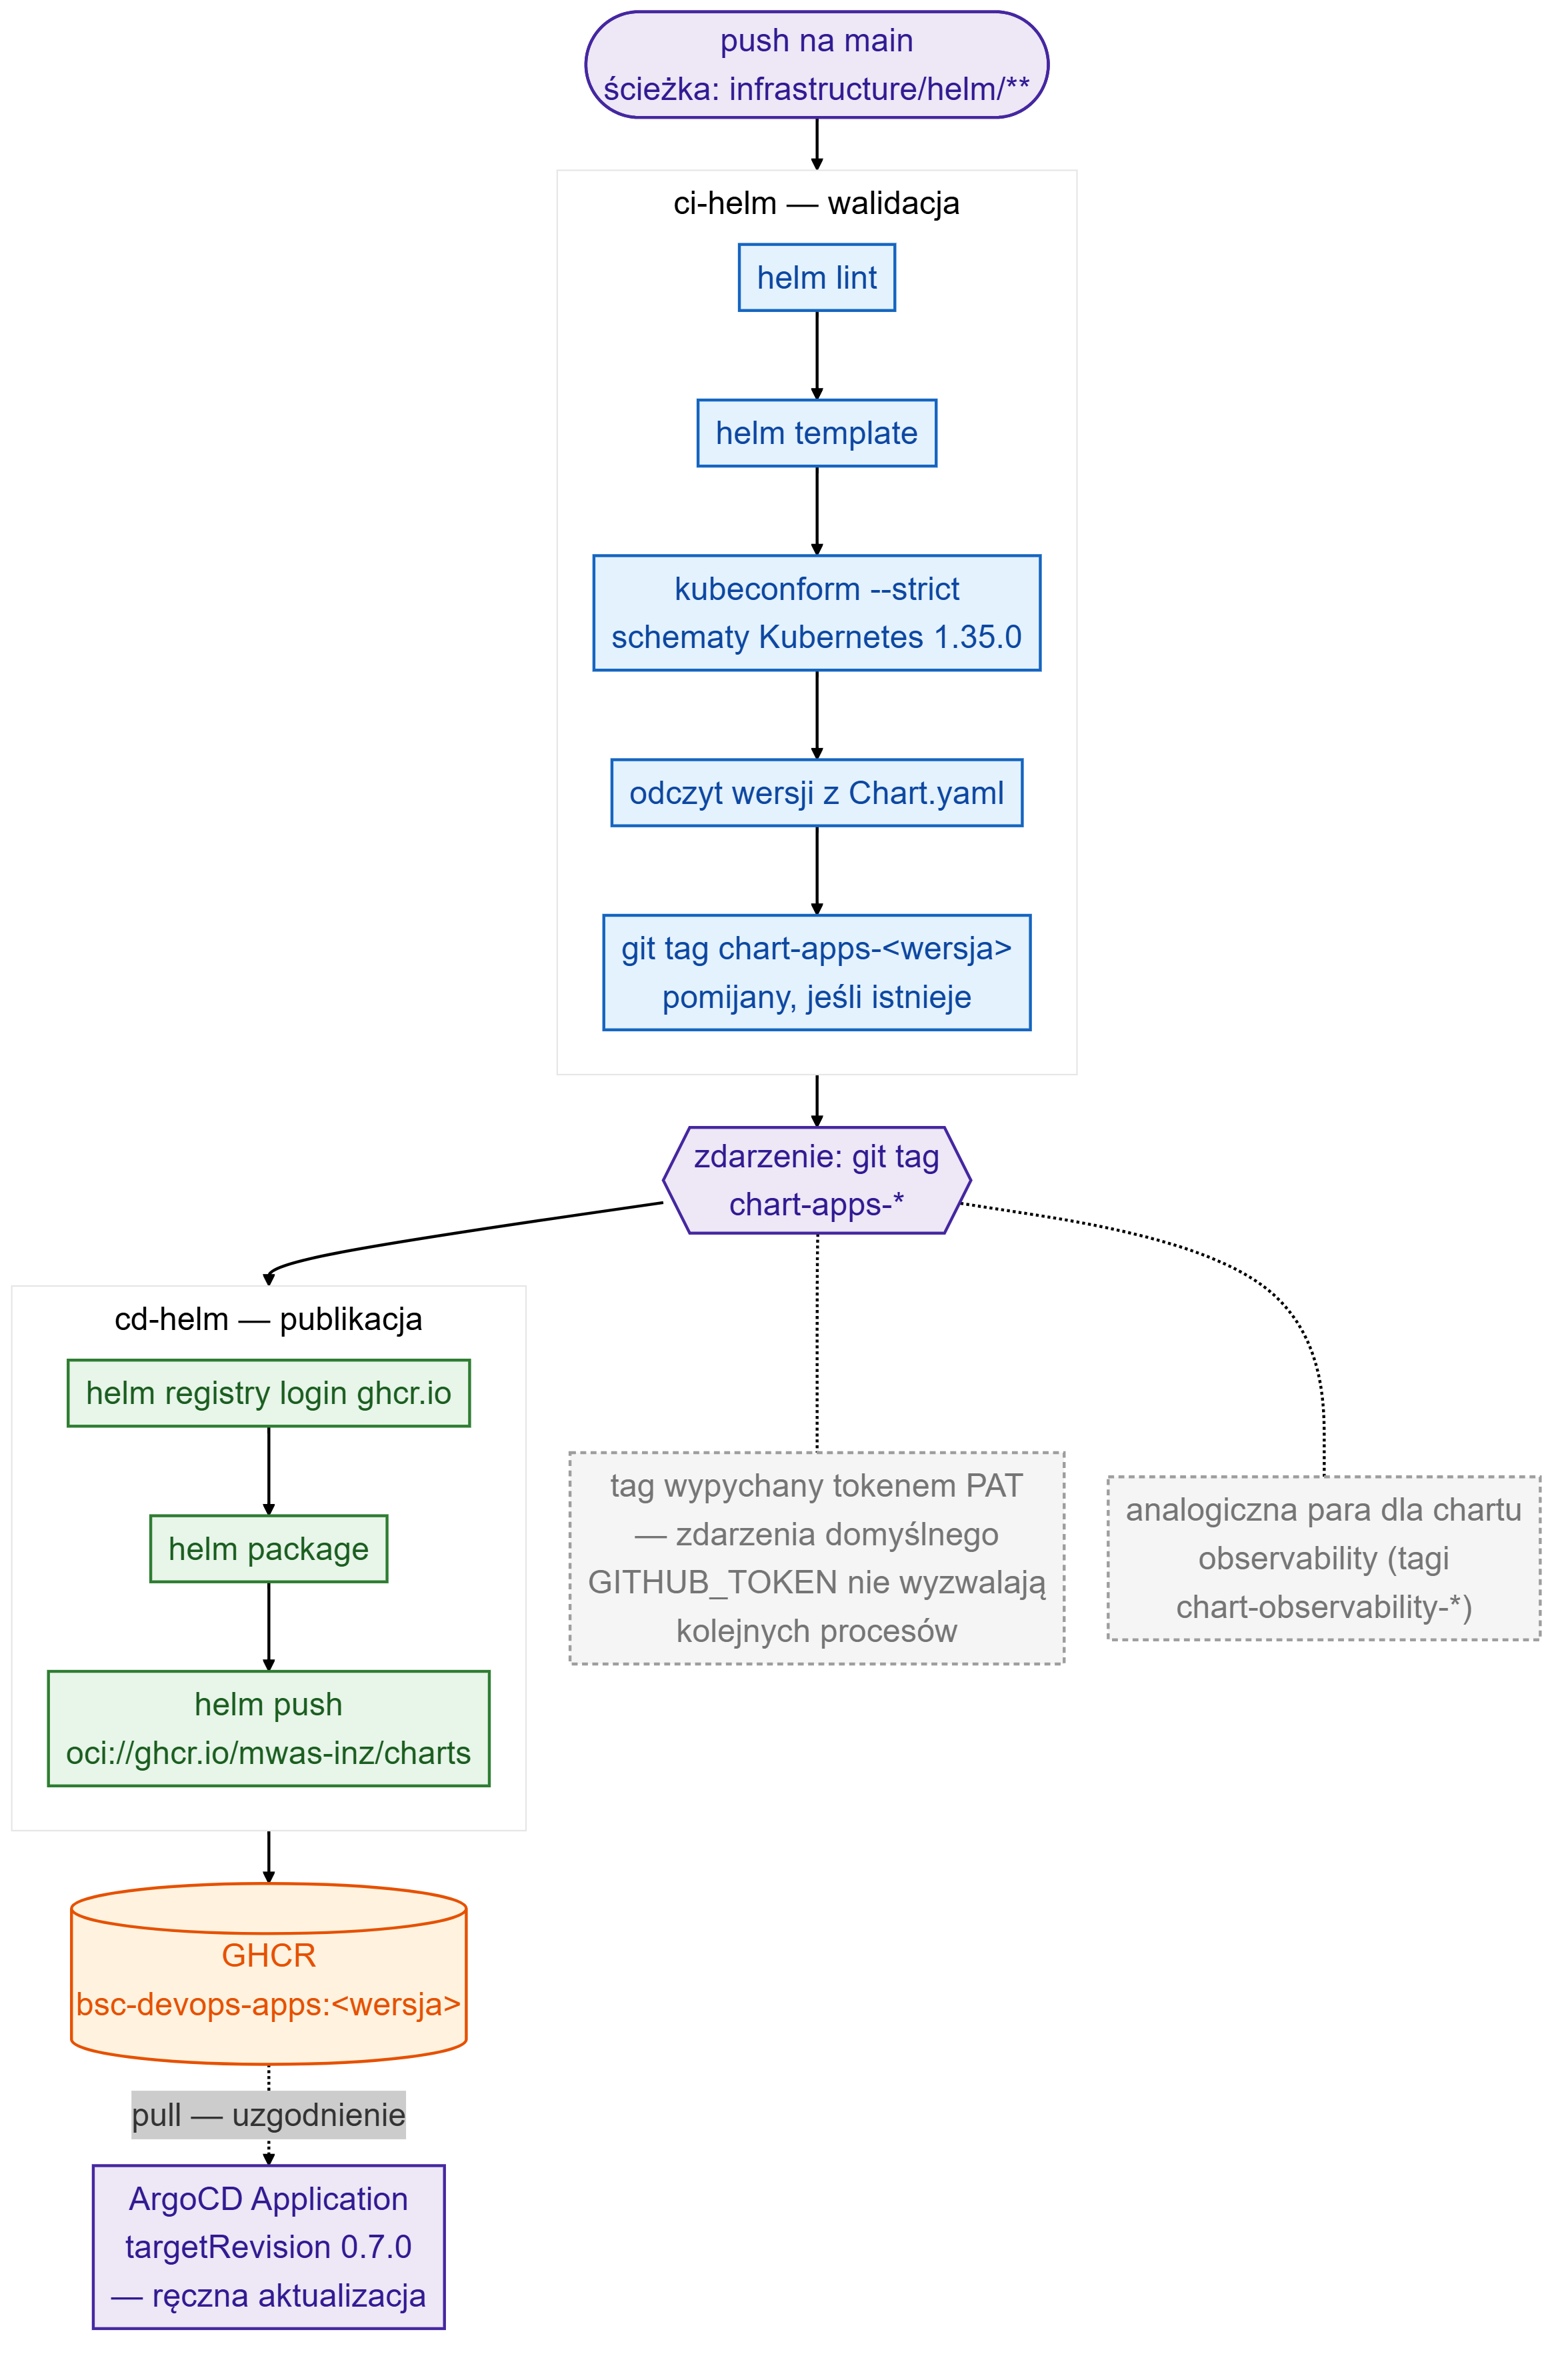
\includegraphics[width=\textwidth]{img/diagrams/06-release/release-01-flow-chart-release.png}
    \caption{Dwuetapowy proces publikacji chartu --- walidacja (\texttt{ci-helm}) oddzielona od publikacji (\texttt{cd-helm}) niezmiennym git tagiem \texttt{chart-apps-<wersja>}; artefakt OCI konsumowany przez ArgoCD według przypiętej wersji (opracowanie własne).}
    \label{fig:chart-release}
\end{figure}

\subsection{Etap Deploy}
Faza wdrożenia (\textit{Deploy}) odpowiada za przeniesienie artefaktów na środowisko uruchomieniowe oraz zapewnienie odpowiedniej infrastruktury.

\subsubsection{Środowisko uruchomieniowe: Kubernetes (k3d)}
Głównym środowiskiem uruchomieniowym mikroserwisów jest klaster \textbf{Kubernetes} (K8s) — otwartoźródłowy system automatyzacji wdrażania, skalowania i zarządzania skonteneryzowanymi aplikacjami. Pełni rolę orkiestratora: dba o to, aby zdefiniowana liczba instancji aplikacji (podów) była zawsze uruchomiona i dostępna, a w przypadku awarii automatycznie je restartuje. Lokalne klastry Kubernetes oferują niemal pełną kompatybilność z produkcyjnymi klastrami chmurowymi (EKS, GKE), co pozwala testować manifesty, polityki sieciowe i mechanizmy skalowania bezpośrednio na maszynie programisty.

\begin{techcard}{Kubernetes}

\textbf{Opis:} Kubernetes (K8s) to otwartoźródłowy system automatyzacji wdrażania, skalowania i zarządzania skonteneryzowanymi aplikacjami. Pełni rolę orkiestratora, dbając o to, aby zdefiniowana liczba instancji aplikacji (podów) była zawsze uruchomiona i dostępna dla użytkowników.

\textbf{Dobre nawyki:}
\begin{itemize}
  \item \textbf{Zarządzanie zasobami:} Obowiązkowe definiowanie \texttt{requests} (zasoby gwarantowane) i \texttt{limits} (maksymalne zużycie) zapobiega wzajemnemu zagłuszaniu się usług (efekt \textit{noisy neighbor}).
  \item \textbf{Sondy stanu podów:} \texttt{livenessProbe} (czy kontener żyje) oraz \texttt{readinessProbe} (czy może przyjmować ruch) są kluczowe dla samonaprawialności klastra i bezprzestojowych wdrożeń (\textit{Rolling Updates}).
  \item \textbf{Podejście deklaratywne (GitOps):} Konfiguracja przechowywana w repozytorium i nakładana przez \texttt{kubectl apply}, a nie komendy imperatywne.
  \item \textbf{Network Policies:} Domyślne ograniczanie komunikacji między podami do niezbędnego minimum -- zasada \textit{Zero Trust}.
\end{itemize}

\textbf{Rola w projekcie:} Kubernetes stanowi docelowe środowisko uruchomieniowe. O ile Docker pozwala stworzyć obraz, o tyle Kubernetes odpowiada za to, by ten obraz funkcjonował w klastrze, był dostępny pod konkretnym adresem i automatycznie restartował się w przypadku awarii.

\end{techcard}

\begin{lstlisting}[language=yaml, caption={Manifest Kubernetes Deployment z sondami kondycji i limitami zasobów (infrastructure/k8s/users-deployment.yaml)}, label={lst:k8s-deployment}]
apiVersion: apps/v1
kind: Deployment
metadata:
  name: users-deployment
spec:
  replicas: 3
  selector:
    matchLabels:
      app: users
  template:
    metadata:
      labels:
        app: users
      annotations:
        prometheus.io/scrape: "true"
        prometheus.io/path: /q/metrics
        prometheus.io/port: "8080"
    spec:
      containers:
      - name: users
        image: mateuszwas/users:1.0.0
        ports:
        - containerPort: 8080
        resources:
          requests:
            memory: "64Mi"
            cpu: "50m"
          limits:
            memory: "256Mi"
            cpu: "500m"
        livenessProbe:
          httpGet:
            path: /q/health/live
            port: 8080
        readinessProbe:
          httpGet:
            path: /q/health/ready
            port: 8080
\end{lstlisting}

W części praktycznej lokalny klaster uruchamia narzędzie \textbf{k3d} — cienka warstwa opakowująca \textbf{k3s} (certyfikowaną przez CNCF dystrybucję Kubernetes) działającą wewnątrz kontenerów Docker. Kluczowym wymaganiem było dotarcie do Ingressu bezpośrednio z hosta bez dodatkowych komend. Alternatywa — \textbf{minikube} z driverem Docker — wymaga uruchomienia \texttt{minikube tunnel} w osobnym terminalu, by ruch z hosta docierał do zasobów Ingress. k3d rozwiązuje ten problem przez mapowanie portów już na etapie tworzenia klastra:

\begin{lstlisting}[language=bash, caption={Tworzenie klastra k3d z mapowaniem portów Ingress (infrastructure/k3d/cluster-create.sh)}, label={lst:k3d-create}]
k3d cluster create bsc-devops \
  --agents 2 \
  --port "80:80@loadbalancer" \
  --port "443:443@loadbalancer"
\end{lstlisting}

Powyższe polecenie mapuje port 80 hosta na load balancer k3d, dzięki czemu każdy zasób Ingress jest natychmiast dostępny pod adresem \texttt{http://localhost}. Klaster startuje w czasie poniżej 30 sekund (w porównaniu do 1--2 minut dla minikube).

\begin{itemize}
    \item \textbf{Wbudowany kontroler Ingress:} k3s domyślnie instaluje \textbf{Traefik} jako kontroler Ingress — nie wymaga ręcznego instalowania dodatków.
    \item \textbf{Wiele węzłów:} Flaga \texttt{--agents N} pozwala tworzyć klastry wielowęzłowe, umożliwiając testowanie zachowania schedulera zbliżonego do środowisk produkcyjnych.
    \item \textbf{Import obrazów lokalnych:} Polecenie \texttt{k3d image import <obraz> -c bsc-devops} ładuje lokalne obrazy Docker bezpośrednio do klastra bez potrzeby wypychania ich do zewnętrznego rejestru.
\end{itemize}

\begin{techcard}{k3d}

\textbf{Opis:} k3d to narzędzie uruchamiające klastry \textbf{k3s} (lekkiej dystrybucji Kubernetes certyfikowanej przez CNCF) wewnątrz kontenerów Docker. Każdy węzeł klastra jest osobnym kontenerem, a porty load balancera są mapowane na host już w momencie tworzenia klastra. Rozwiązuje to główną bolączkę alternatywnych narzędzi lokalnych -- konieczność uruchamiania dodatkowych procesów tunelujących ruch Ingress.

\textbf{Dobre nawyki:}
\begin{itemize}
  \item \textbf{Mapowanie portów przy tworzeniu:} Flagi \texttt{--port} należy podać w poleceniu \texttt{k3d cluster create} -- nie da się ich dodać do działającego klastra bez jego rekonstrukcji.
  \item \textbf{Import obrazów lokalnych:} Zamiast wypychać obraz do zewnętrznego rejestru podczas iteracji deweloperskiej, należy użyć \texttt{k3d image import <obraz> -c <klaster>} -- ładuje obraz bezpośrednio do containerd w węzłach klastra.
  \item \textbf{Domyślny Ingress: Traefik:} k3s dostarcza Traefik zamiast nginx; manifesty Ingress muszą używać \texttt{ingressClassName: traefik}.
  \item \textbf{Wielowęzłowość:} Dla testów zbliżonych do produkcji warto dodać agentów (\texttt{--agents 2}), by sprawdzić zachowanie schedulera przy ograniczeniach \texttt{affinity}/\texttt{tolerations}.
\end{itemize}

\textbf{Rola w projekcie:} k3d stanowi lokalne środowisko deweloperskie i demonstracyjne dla całego stosu mikroserwisów. Zastąpił minikube ze względu na natywne mapowanie portów Ingress (brak \texttt{minikube tunnel}), czas startu klastra poniżej 30 sekund oraz pełną skryptowalność tworzenia klastra jedną komendą CLI.

\end{techcard}

\subsubsection{Automatyzacja wdrożeń: GitOps (ArgoCD)}
Zamiast tradycyjnych narzędzi \textit{Configuration Management} (jak Ansible), zdecydowano się na podejście \textbf{GitOps} przy użyciu narzędzia \textbf{ArgoCD} (ADR-0013). GitOps zakłada, że repozytorium Git jest jedynym źródłem prawdy o stanie infrastruktury -- kontroler stale monitoruje zmiany w chartach Helm i automatycznie synchronizuje stan klastra z definicją w kodzie, eliminując potrzebę ręcznego wykonywania poleceń \texttt{kubectl} z poziomu CI/CD.

\begin{techcard}{ArgoCD}

\textbf{Opis:} ArgoCD to deklaratywny kontroler GitOps dla Kubernetes, będący projektem CNCF o statusie \textit{graduated}. Działa w modelu \textbf{pull-based}: nasłuchuje zmian w repozytorium Git lub rejestrze OCI i automatycznie synchronizuje stan klastra do zdefiniowanego tam stanu docelowego. Centralną abstrakcją jest zasób \texttt{Application}, który wiąże źródło (chart Helm, katalog manifestów) z docelowym klastrem i przestrzenią nazw. Wbudowany interfejs webowy pozwala w czasie rzeczywistym obserwować drzewo zasobów aplikacji oraz historię wdrożeń.

\textbf{Dobre nawyki:}
\begin{itemize}
  \item \textbf{Automated sync z \texttt{selfHeal}:} Włączenie \texttt{selfHeal: true} gwarantuje, że każda ręczna zmiana w klastrze zostanie natychmiast cofnięta -- klaster jest zawsze zgodny z tym, co opisuje Git.
  \item \textbf{\texttt{prune: true} z rozwagą:} Automatyczne usuwanie zasobów odłączonych od charta skraca dług konfiguracyjny, ale wymaga pewności, że wszystkie zasoby są zarządzane przez ArgoCD.
  \item \textbf{Application CRD w Git:} Plik \texttt{gitops/application.yaml} powinien być przechowywany w repozytorium obok charta -- cały opis dostawy jest wówczas wersjonowany i audytowalny.
  \item \textbf{Pinowanie \texttt{targetRevision}:} Używanie konkretnego numeru wersji charta (nie \texttt{latest}) zapewnia powtarzalność wdrożeń i pełną historię zmian.
\end{itemize}

\textbf{Rola w projekcie:} ArgoCD zamyka pętlę CI/CD: GitHub Actions buduje obraz, publikuje chart do GHCR, a ArgoCD automatycznie wykrywa nową wersję charta i synchronizuje klaster k3d. Zasób \texttt{Application} wskazuje na chart \texttt{bsc-devops} w GHCR i celuje w lokalny klaster k3d. Wbudowany interfejs webowy dostarcza wizualizację drzewa zasobów przydatną jako materiał ilustracyjny pracy.

\end{techcard}

\begin{lstlisting}[language=yaml, caption={ArgoCD Application CRD -- deklaracja dostawy charta \texttt{bsc-devops} z GHCR do klastra k3d (gitops/application.yaml)}, label={lst:argocd-application}]
apiVersion: argoproj.io/v1alpha1
kind: Application
metadata:
  name: bsc-devops
  namespace: argocd
spec:
  project: default
  source:
    repoURL: ghcr.io/mateuszwas/charts   # OCI Helm registry (GHCR)
    chart: bsc-devops
    targetRevision: "0.5.0"
    helm:
      valueFiles:
        - values.yaml
  destination:
    server: https://kubernetes.default.svc
    namespace: bsc-devops
  syncPolicy:
    automated:
      prune: true      # usuwa zasoby usunięte z charta
      selfHeal: true   # cofa ręczne zmiany niezgodne z Gitem
    syncOptions:
      - CreateNamespace=true
\end{lstlisting}

\subsection{Etap Operate}
Faza operacyjna (\textit{Operate}) obejmuje utrzymanie aplikacji w~środowisku produkcyjnym oraz zarządzanie usługami wspierającymi (bazami danych, brokerami wiadomości).
Strukturę utrzymywanego środowiska przedstawia rysunek~\ref{fig:infrastructure}: cztery przestrzenie nazw (ang. \textit{namespace}) klastra pełnią cztery odrębne role --- platformową (\texttt{kube-system}: Traefik jako jedyny punkt wejścia HTTP oraz kontroler Sealed Secrets), dostarczania (\texttt{argocd}), aplikacyjną (\texttt{bsc-devops}) i~obserwacyjną (\texttt{observability}).

\begin{figure}[H]
    \centering
    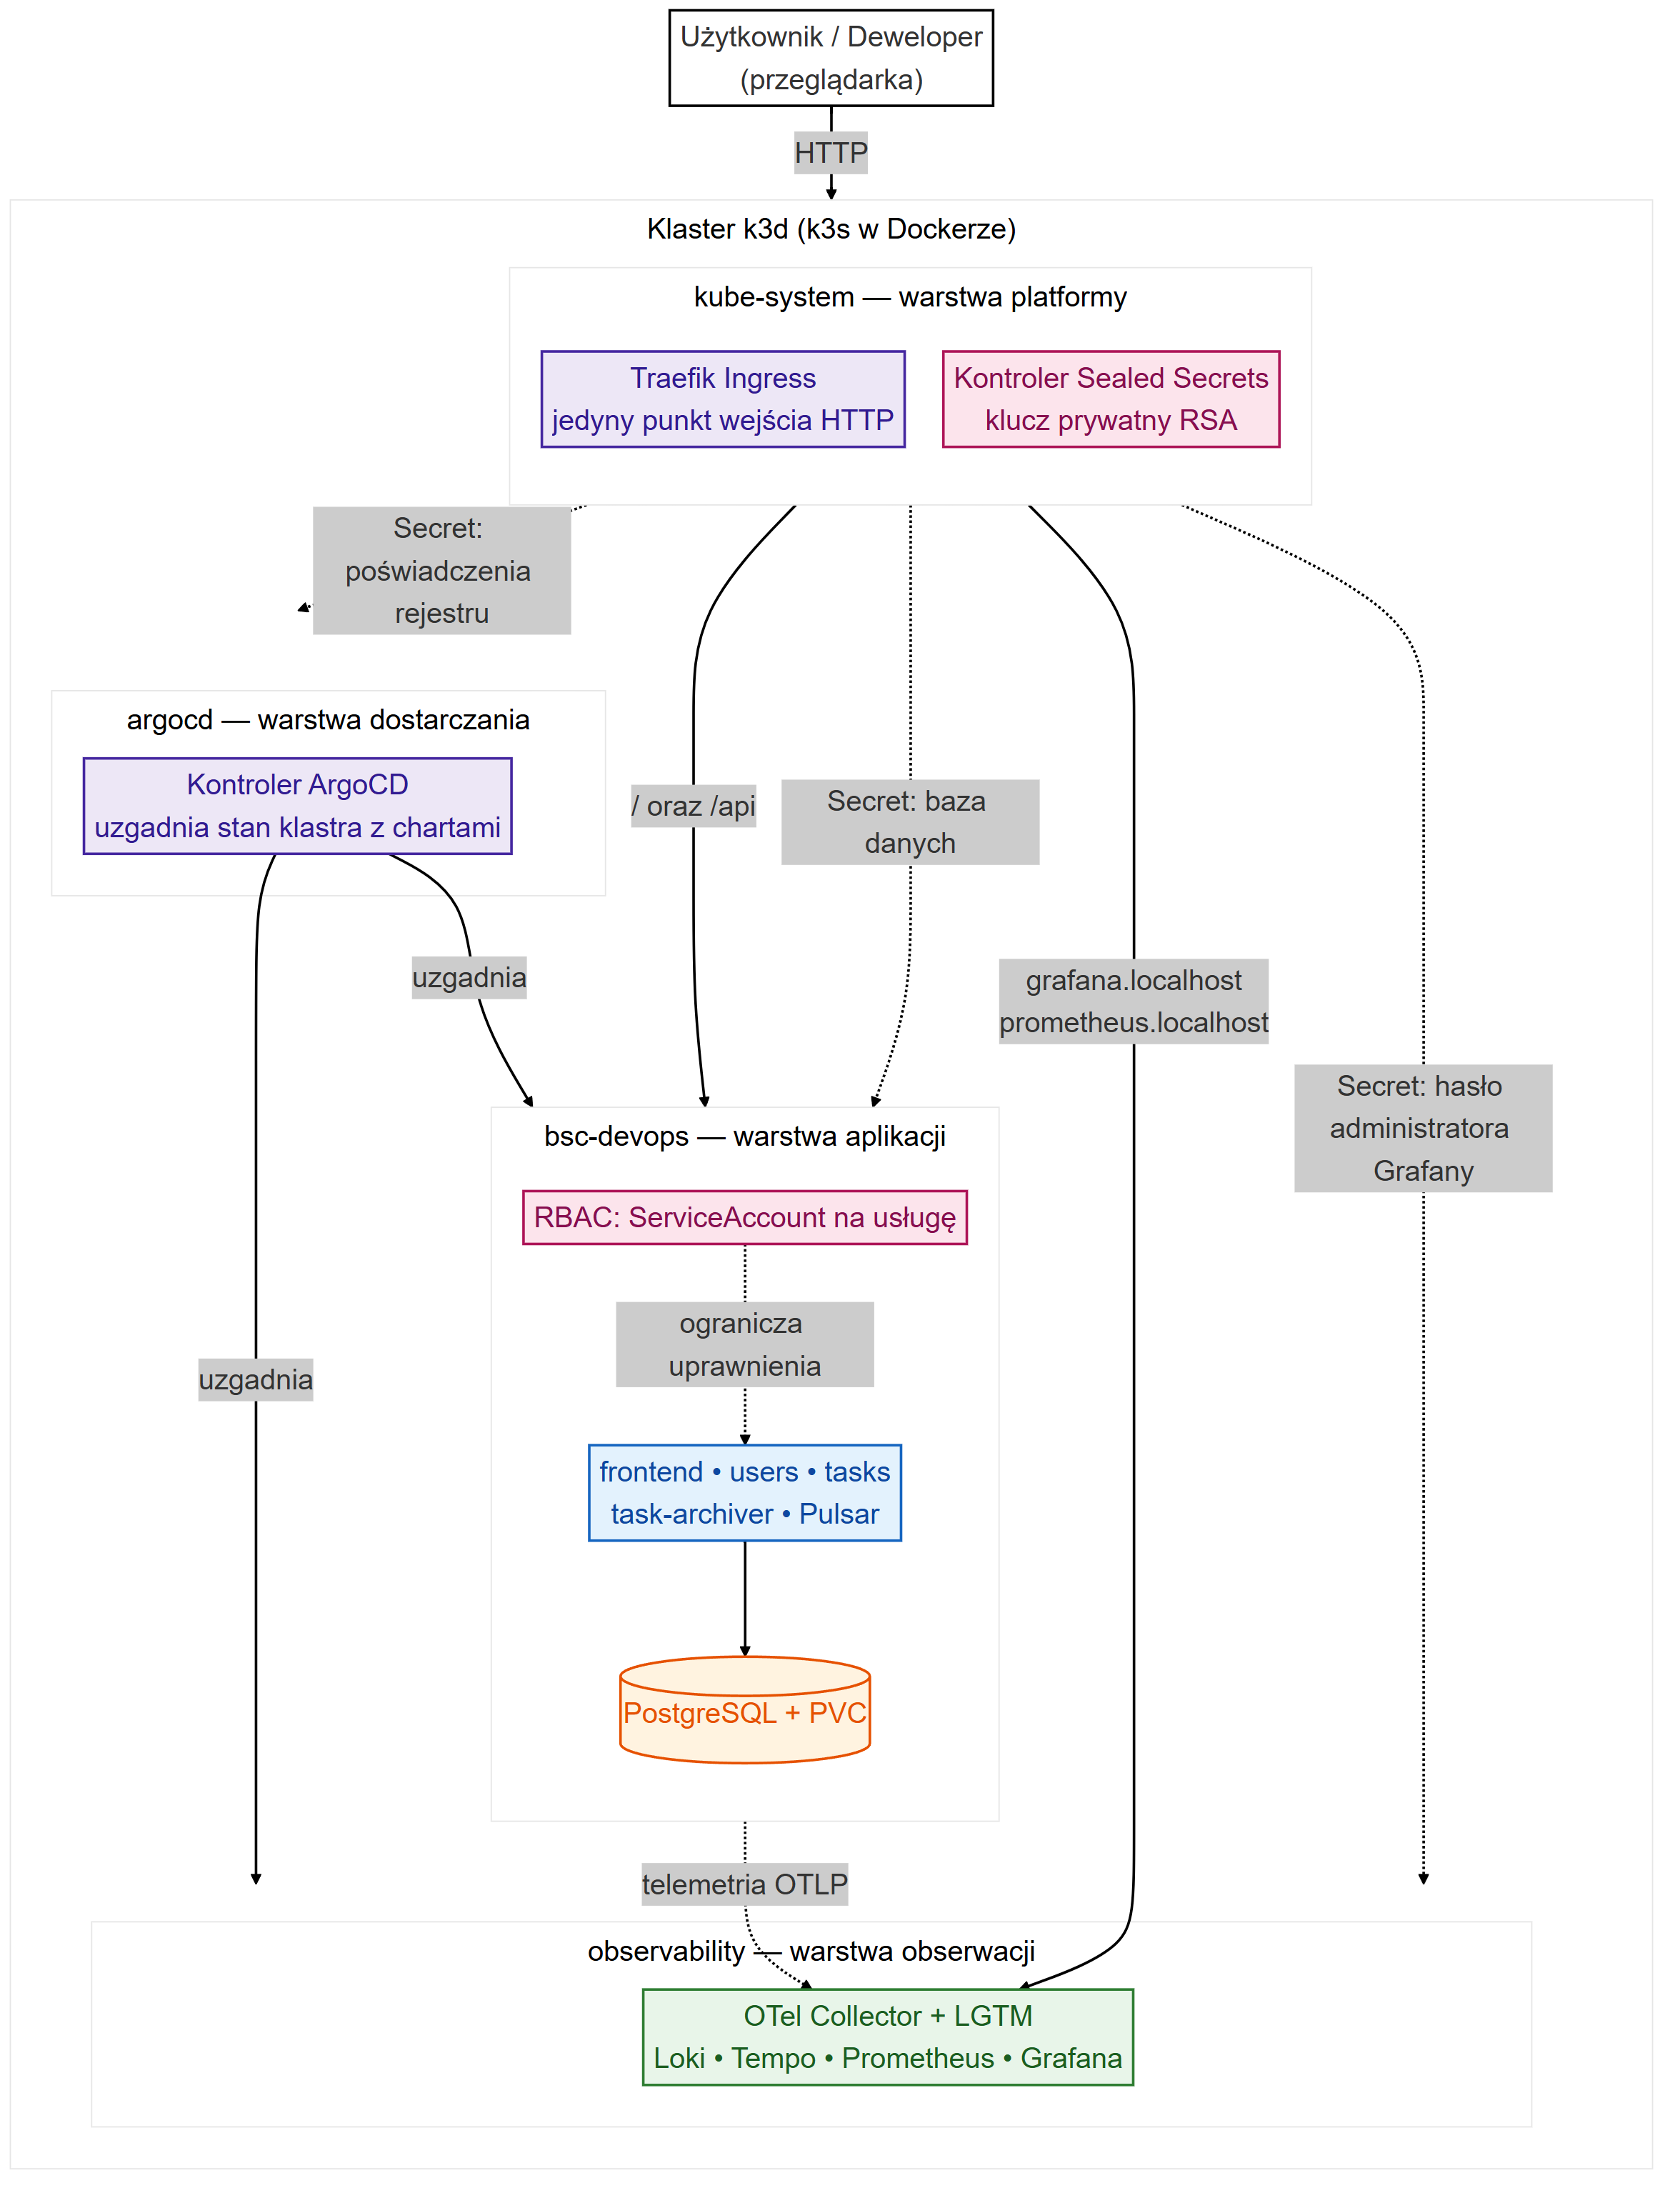
\includegraphics[width=0.95\textwidth]{img/diagrams/08-operate/operate-01-infrastructure.png}
    \caption{Infrastruktura klastra --- cztery przestrzenie nazw, cztery role: platforma, dostarczanie, aplikacje i~obserwacja; kontroler Sealed Secrets odszyfrowuje sekrety do trzech przestrzeni (opracowanie własne).}
    \label{fig:infrastructure}
\end{figure}

\subsubsection{Usługi wspierające w~klastrze}
Zgodnie z~założeniem o~pełnej odtwarzalności środowiska w~modelu lokalnym, zdecydowano się na uruchomienie odpowiedników usług chmurowych bezpośrednio wewnątrz klastra Kubernetes przy użyciu gotowych chartów Helm.
\begin{itemize}
    \item \textbf{Baza danych: PostgreSQL (zamiast AWS RDS):} Dane mikroserwisów są przechowywane w~relacyjnej bazie danych PostgreSQL. W~klastrze lokalnym baza ta działa jako kontener z~zamontowanym wolumenem trwałym (ang. \textit{Persistent Volume}), co zapewnia trwałość danych mimo restartów kontenerów.
    \item \textbf{Broker wiadomości: Apache Pulsar (zamiast np. Amazon MSK):} Komunikacja zdarzeniowa między mikroserwisami odbywa się przez tematy brokera Apache Pulsar uruchomionego w~klastrze; w~środowisku chmurowym rolę tę przejęłaby usługa zarządzana.
\end{itemize}

Ten sam wzorzec zastępowania dotyczy pozostałych elementów platformy. Rysunek~\ref{fig:aws-equivalent} zestawia komponenty uruchomione lokalnie z~ich zarządzanymi odpowiednikami w~chmurze AWS --- wariant chmurowy pozostaje propozycją, świadomie niezaimplementowaną w~ramach pracy, ilustrującą jednak niezależność platformy od konkretnego dostawcy.

\begin{figure}[H]
    \centering
    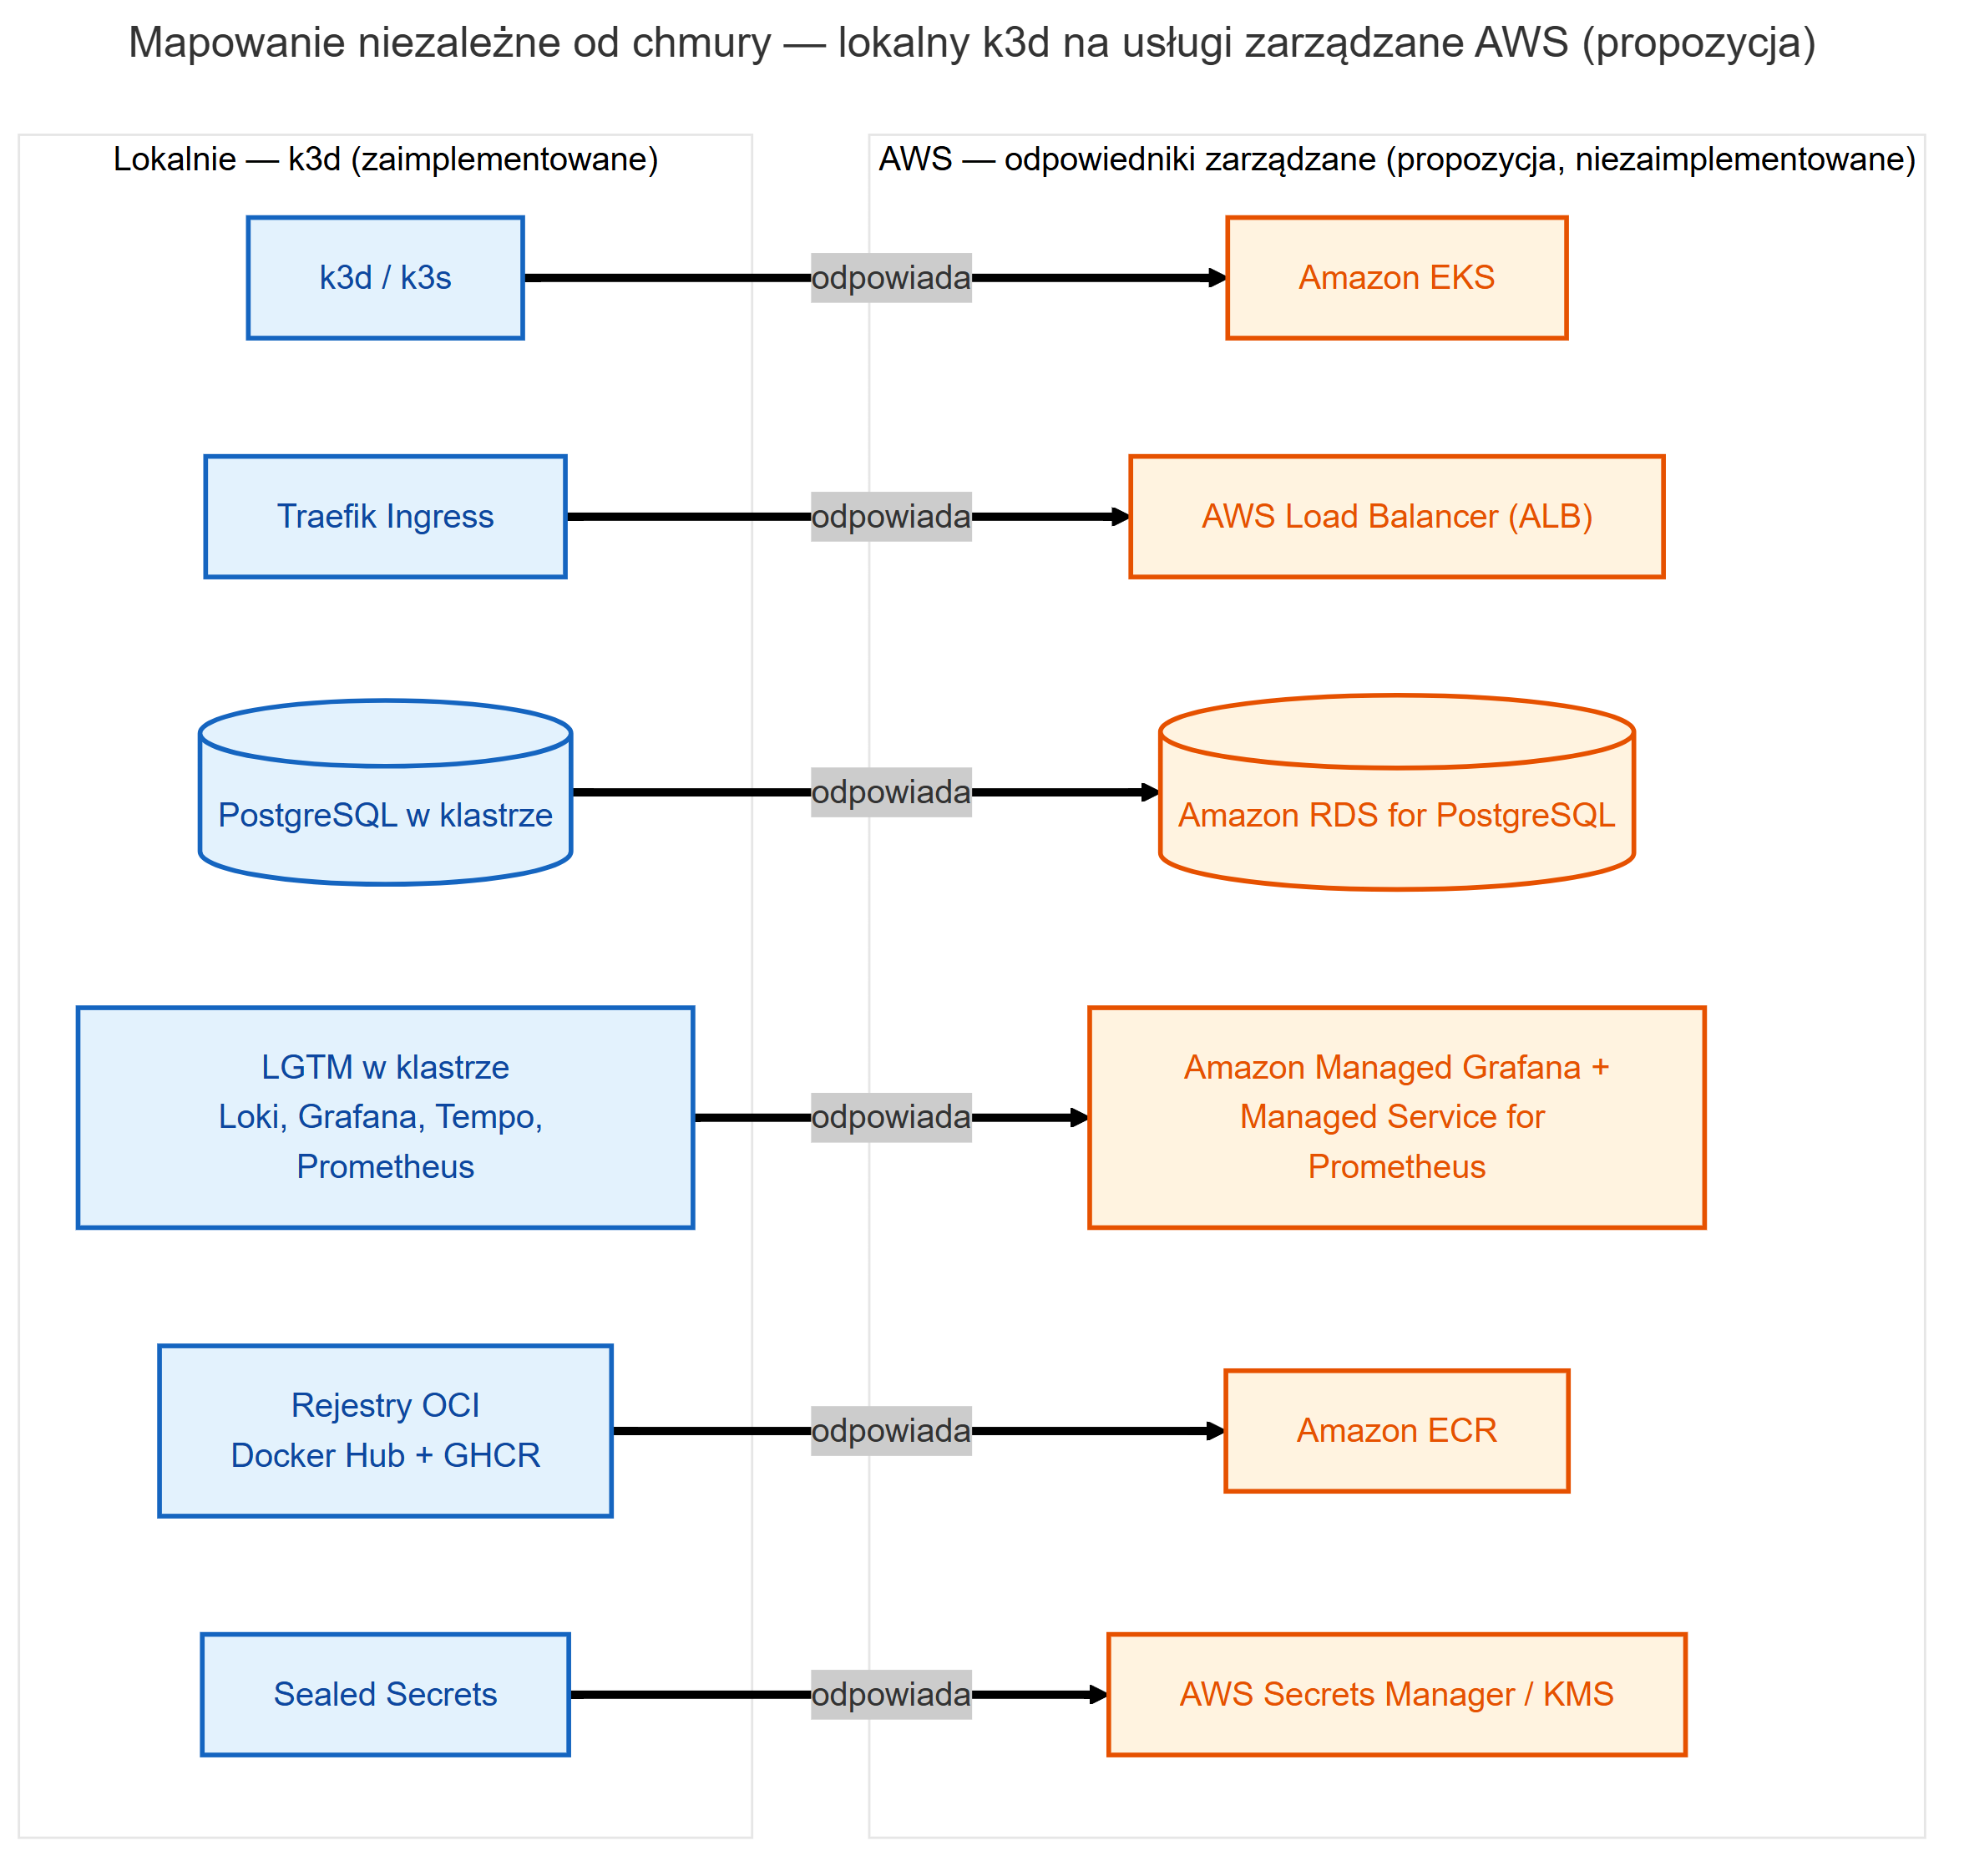
\includegraphics[width=\textwidth]{img/diagrams/08-operate/operate-02-aws-equivalent.png}
    \caption{Mapowanie lokalnego środowiska na zarządzane usługi AWS --- propozycja migracji ilustrująca niezależność od dostawcy; wariant chmurowy nie był implementowany (opracowanie własne).}
    \label{fig:aws-equivalent}
\end{figure}

\subsubsection{Zarządzanie zasobami: Kubernetes}
Kubernetes zarządza cyklem życia wszystkich komponentów, dbając o~ich samonaprawę (ang. \textit{self-healing}) oraz odpowiednie przydzielanie zasobów procesora i~pamięci. Wykorzystanie lokalnego klastra pozwala na demonstrację tych mechanizmów bez generowania kosztów infrastrukturalnych.

\subsection{Etap Monitor + Feedback}
Ostatni etap pętli DevOps zamyka cykl, dostarczając informacji zwrotnej o działaniu systemu. W nowoczesnych architekturach etap ten jest realizowany poprzez koncepcję \textit{Observability}.

\subsubsection{Standard zbierania danych: OpenTelemetry}
Zgodnie z decyzją \textit{ADR-0006}, w całym projekcie zaimplementowano standard \textbf{OpenTelemetry}.
\begin{itemize}
    \item \textbf{Jednolita instrumentacja:} Zamiast oddzielnych bibliotek dla logów, metryk i trace'ów, aplikacje wykorzystują ujednolicony protokół OTLP.
    \item \textbf{OTel Collector:} Centralnym punktem zbierania danych jest komponent Collector, który odbiera telemetrię z aplikacji, przetwarza ją i wysyła do odpowiednich systemów bazodanowych. Pozwala to na całkowite odseparowanie aplikacji od konkretnych dostawców narzędzi monitorujących.
\end{itemize}

\subsubsection{Stos Observability: LGTM}
Jako systemy przechowywania i wizualizacji danych wybrano stos \textbf{LGTM} (ADR-0007):
\begin{itemize}
    \item \textbf{Prometheus (Metrics):} Gromadzi dane numeryczne o wydajności systemu i aplikacji.
    \item \textbf{Loki (Logs):} Przechowuje logi aplikacji w sposób zoptymalizowany pod kątem Kubernetes (wykorzystując te same etykiety co system orkiestracji).
    \item \textbf{Tempo (Traces):} Umożliwia śledzenie rozproszonych zapytań między mikroserwisami, co jest kluczowe w diagnozowaniu problemów wydajnościowych w architekturze rozproszonej.
    \item \textbf{Grafana (Visualization):} Stanowi wspólny interfejs (\textit{Single Pane of Glass}) dla wszystkich powyższych narzędzi. Pozwala na tworzenie interaktywnych pulpitów sterowniczych i korelację danych (np. przejście od wykresu błędu do logów konkretnego kontenera).
\end{itemize}

\subsection{Podsumowanie części praktycznej}
Zaprezentowany ekosystem narzędziowy tworzy spójny proces wytwórczy (\textit{Golden Path}), który minimalizuje nakład pracy ręcznej i ryzyko błędów ludzkich. Integracja poszczególnych etapów — od planowania w systemie Jira, przez automatyczne budowanie i testowanie w GitHub Actions, aż po wdrożenie GitOps i zaawansowane monitorowanie — stanowi kompletną realizację paradygmatu DevOps w architekturze \textit{Cloud Native}. Tak ukształtowane środowisko pozwala deweloperom skupić się na dostarczaniu wartości biznesowej, podczas gdy infrastruktura i procesy pozostają zautomatyzowane, przejrzyste i mierzalne.

\newpage
\section{Podsumowanie i wnioski}
\lipsum[1]

%--------------------------------------------
% Literatura
%--------------------------------------------
\cleardoublepage % Zaczynamy od nieparzystej strony
\printbibliography

%--------------------------------------------
% Spisy (opcjonalne)
%--------------------------------------------
\newpage
\pagestyle{plain}

% Wykaz symboli i skrótów.
% Pamiętaj, żeby posortować symbole alfabetycznie
% we własnym zakresie. Ponieważ mało kto używa takiego wykazu,
% uznałem, że robienie automatycznie sortowanej listy
% na poziomie LaTeXa to za duży overkill.
% Makro \acronymlist generuje właściwy tytuł sekcji,
% w zależności od języka.
% Makro \acronym dodaje skrót/symbol do listy,
% zapewniając podstawowe formatowanie.
% //AB
\vspace{0.8cm}
\acronymlist
\acronym{ADR}{ang. \textit{Architectural Decision Record} -- zapis decyzji architektonicznej}
\acronym{API}{ang. \textit{Application Programming Interface} -- interfejs programowania aplikacji}
\acronym{AOT}{ang. \textit{Ahead-of-Time} -- kompilacja przed czasem wykonania}
\acronym{CD}{ang. \textit{Continuous Delivery} / \textit{Continuous Deployment} -- ciągłe dostarczanie / wdrażanie}
\acronym{CDI}{ang. \textit{Contexts and Dependency Injection} -- wstrzykiwanie zależności}
\acronym{CI}{ang. \textit{Continuous Integration} -- ciągła integracja}
\acronym{CVE}{ang. \textit{Common Vulnerabilities and Exposures} -- rejestr znanych podatności}
\acronym{Dev}{ang. \textit{development} -- wytwarzanie oprogramowania}
\acronym{DORA}{ang. \textit{DevOps Research and Assessment}}
\acronym{EiTI}{Wydział Elektroniki i Technik Informacyjnych}
\acronym{IaC}{ang. \textit{Infrastructure as Code} -- infrastruktura jako kod}
\acronym{IT}{ang. \textit{Information Technology} -- technologie informacyjne}
\acronym{JDK}{ang. \textit{Java Development Kit} -- zestaw narzędzi deweloperskich Java}
\acronym{JVM}{ang. \textit{Java Virtual Machine} -- wirtualna maszyna Java}
\acronym{K8s}{Kubernetes (skrót od: \textit{K}ubernete\textit{s}, 8 liter pomiędzy K i s)}
\acronym{LGTM}{Loki, Grafana, Tempo, Mimir -- stos narzędzi obserwacyjności}
\acronym{Ops}{ang. \textit{operations} -- operacje, utrzymanie systemów}
\acronym{OTLP}{ang. \textit{OpenTelemetry Protocol} -- protokół OpenTelemetry}
\acronym{PW}{Politechnika Warszawska}
\acronym{REST}{ang. \textit{Representational State Transfer} -- styl architektury API}
\acronym{SRE}{ang. \textit{Site Reliability Engineering} -- inżynieria niezawodności}
\acronym{YAML}{ang. \textit{YAML Ain't Markup Language} -- format serializacji danych}

\listoffigurestoc     % Spis rysunków.
\vspace{1cm}          % vertical space
\listoftablestoc      % Spis tabel.
\vspace{1cm}          % vertical space
\listofappendicestoc  % Spis załączników

% Załączniki
\newpage
\appendix{Nazwa załącznika 1}
\lipsum[1-8]

\newpage
\appendix{Nazwa załącznika 2}
\lipsum[1-4]

% Używając powyższych spisów jako szablonu,
% możesz tu dodać swój własny wykaz bądź listę,
% np. spis algorytmów.

\end{document} % Dobranoc.
